% In your .tex file
% !TEX program = latex
%  A simple AAU report template.
%  2014-09-13 v. 1.1.0
%  Copyright 2010-2014 by Jesper Kjær Nielsen <jkn@es.aau.dk>
%
%  This is free software: you can redistribute it and/or modify
%  it under the terms of the GNU General Public License as published by
%  the Free Software Foundation, either version 3 of the License, or
%  (at your option) any later version.
%
%  This is distributed in the hope that it will be useful,
		%  but WITHOUT ANY WARRANTY; without even the implied warranty of
%  MERCHANTABILITY or FITNESS FOR A PARTICULAR PURPOSE.  See the
%  GNU General Public License for more details.
%
%  You can find the GNU General Public License at <http://www.gnu.org/licenses/>.
%
%  A simple AAU report template.
%  2014-09-13 v. 1.1.0
%  Copyright 2010-2014 by Jesper Kjær Nielsen <jkn@es.aau.dk>
%
%  This is free software: you can redistribute it and/or modify
%  it under the terms of the GNU General Public License as published by
%  the Free Software Foundation, either version 3 of the License, or
%  (at your option) any later version.
%
%  This is distributed in the hope that it will be useful,
%  but WITHOUT ANY WARRANTY; without even the implied warranty of
%  MERCHANTABILITY or FITNESS FOR A PARTICULAR PURPOSE.  See the
%  GNU General Public License for more details.
%
%  You can find the GNU General Public License at <http://www.gnu.org/licenses/>.
%
\documentclass[11pt,twoside,a4paper,openright]{memoir}
%%%%%%%%%%%%%%%%%%%%%%%%%%
%% COMMAND DEACTIVATION %%
%%%%%%%%%%%%%%%%%%%%%%%%%%

\let\added\undefined
\let\deleted\undefined


%%%%%%%%%%%%%%
%% PACKAGES %%
%%%%%%%%%%%%%%


%%% Initial things %%%
% Fix various issues with LaTeX2e
\usepackage{fixltx2e}
% Font package
\usepackage{fourier}
% Index
\usepackage{makeidx}
\makeindex


%%% Translations and character encodings %%%
% Enable use of several characters, including æ, ø and å
\usepackage[utf8]{inputenc}
%  language
\usepackage[english]{babel}
% Use PostScript fonts instead of bitmap ones. Also does other stuff.
\usepackage[T1]{fontenc}
% Various LaTeX symbols
\usepackage{latexsym}
% Wider selection of colours
\usepackage[pdftex,dvipsnames,table]{xcolor}  % Coloured text etc.% Improved element justification
\usepackage{ragged2e}
% Font improvements
\usepackage{fix-cm}
% Enables inclusion of PDF files
\usepackage{pdfpages}
% Enables various forms of lines, like double-underlining (\uuline{})
\usepackage[normalem,normalbf]{ulem}
% Sets the tolerance for distance between words, determining when to hyphenate.
\pretolerance=2500


%%% Figures and tables (Floats) %%%
% Ensures that floats won't appear -before- the place where they're added
\usepackage{flafter}
% Enable multi-rows and -columns
\usepackage{multirow}
\usepackage{multicol}
% Double, horizontal lines
\usepackage{hhline}
% Enables coloured tables
\usepackage{colortbl}
% Gives improved control over placement of floats
% \begin{figure}[!h] % Won't be floating
\usepackage{here}
% Wrap text around figures
\usepackage{wrapfig}
% Wrap text around tables
\usepackage{floatflt}
% Enables the \FloatBarrier command
\usepackage{placeins}
% Rotation of figures
\usepackage{rotating}
% Framed boxes
\usepackage{framed}
% Booktabs - Fancy tables
\usepackage{booktabs}
% Enables inclusion of PDF documents of version 1.6+
%\pdfoptionpdfminorversion=6


%%% Mathematic formulas %%%
% AMS math
%\usepackage{amsmath}
%\usepackage{amssymb}
% Extra fonts (for math, I think)
\usepackage{stmaryrd}
% Access text symbols
\usepackage{textcomp}
% Extend AMS
%\usepackage{mathtools}
%\usepackage{cancel}
% Use theorems in your document
% The ntheorem package is also used for the example environment
% When using thmmarks, amsmath must be an option as well. Otherwise \eqref doesn't work anymore.
%\usepackage[framed,amsmath,thmmarks]{ntheorem}
% Pretty fractions, just because
%\usepackage{nicefrac}


%%% Graphics %%%
% Various image-commands
\usepackage{eso-pic}
% Use JPEG and PNG images
\usepackage{array,graphicx}
\DeclareGraphicsExtensions{.pdf,.png,.jpg}
\graphicspath{{./images/}}
%Wrapping Images
\usepackage{wrapfig}


%%% Text stuff %%%
% Filler text
%\usepackage{lipsum}
% Page counting
%\usepackage{totpages}
% Acronyms
%\usepackage{acronym}
%avoid widows
%\widowpenalty10000


%%% Source Code Stuff %%%
% Adds \lstinline!code there!, where !! are delimeters not used in the code
% Adds the environment: lstlisting
% Adds command \lstinputlisting[options]{filename.ext}
% More info in manual.
%\usepackage{listings}
%\lstloadlanguages{[Sharp]C,XML,SQL}
%\lstset{numbers=left,
%        numberstyle=\tiny,
%        stepnumber=2,
%        numbersep=5pt,
%        frame=tb,
%        inputencoding=utf8,
%        tabsize=2,
%        extendedchars=true,
%        language=[Sharp]C}

\usepackage{color}
\definecolor{bluekeywords}{rgb}{0.13,0.13,1}
\definecolor{greencomments}{rgb}{0,0.5,0}
\definecolor{redstrings}{rgb}{0.9,0,0}

\usepackage{courier}

\usepackage{listings}

\lstdefinelanguage{JavaScript}{
  keywords={typeof, new, true, false, catch, function, return, null, catch, switch, var, if, in, while, do, else, case, break},
  keywordstyle=\color{blue}\bfseries,
  ndkeywords={class, export, boolean, throw, implements, import, this},
  ndkeywordstyle=\color{darkgray}\bfseries,
  identifierstyle=\color{black},
  sensitive=false,
  comment=[l]{//},
  morecomment=[s]{/*}{*/},
  commentstyle=\color{purple}\ttfamily,
  stringstyle=\color{red}\ttfamily,
  morestring=[b]',
  morestring=[b]"
}


\lstset{language=[Sharp]C,
  captionpos=b,            
  columns=fixed,     
  numbers=left,
  numberstyle=\tiny,
  showspaces=false,
  showtabs=false,
  breaklines=true,
  inputencoding=utf8,
  showstringspaces=false,
  breakatwhitespace=true,
  escapeinside={(*@}{@*)},
  commentstyle=\color{greencomments},
  keywordstyle=\color{bluekeywords},
  stringstyle=\color{redstrings},
  basicstyle=\ttfamily\small,
  literate={ø}{{\o}}1
  		   {æ}{{\ae}}1
  		   {å}{{\aa}}1
  		   {Ø}{{\O}}1
  		   {Æ}{{\AE}}1
  		   {Å}{{\AA}}1
         {§}{{\S}}1
}

\lstdefinestyle{make}{tabsize=4}

%%% References, bibtex and URLs %%%
% Post URLs. Allows breaking at hyphens to help avoid long links.
\usepackage[hyphens]{url}
% Better cross references
\usepackage[danish]{varioref}
% Enable natbib citation styles
\usepackage[numbers]{natbib}
% Define a new 'leo' style for URL package, that will use a smaller font
\makeatletter
\def\url@leostyle{%
  \@ifundefined{selectfont}{\def\UrlFont{\sf}}{\def\UrlFont{\small\ttfamily}}
}
\makeatother
% And of course, use this new style
\urlstyle{leo}




%%% Floats %%%
% Not entirely sure why I need this yet
\let\newfloat\relax
\usepackage{float}
% Enables usage of \subcaption, \subtop and \subbottom
\newsubfloat{figure}


%%% Todo Stuff %%%
% Insert needed corrections with \fixme{..}, which will cause an error during compile, if any are present once 'draft'
% is replaced with 'final'
\usepackage[footnote,draft,english,silent,nomargin]{fixme}
\fxsetup{layout={footnote,marginclue,index},innerlayout={inline,index}}


%%% Changes Markup %%%
% Markup changes of varying types.
% Adds the commands:
%  - \added[id=(author id), remark={remark text}]{new text}
%  - \deleted[id=(author id), remark={remark text}]{old text}
%  - \replaced[id=(author id), remark={remark text}]{new text}{old text}
\usepackage[xcolor,authormarkup=footnote]{changes}
% Adds the commands:
%  - \cbstart
%  - \cbend
%  - \cbdelete
%  - Environment: changebar
\usepackage[outerbars,xcolor]{changebar}
\cbcolor{red}



%%%%%%%%%%%%%%%%%%%%%%%
%% DOCUMENT SETTINGS %%
%%%%%%%%%%%%%%%%%%%%%%%


%%% Margins %%%
% \setlrmarginsandblock{binding}{edge}{ratio}
\setlrmarginsandblock{2.0cm}{2.0cm}{*}
% \setulmarginsandblock{top}{bottom}{ratio}
\setulmarginsandblock{2.0cm}{2.0cm}{*}
% Performs various calculations and makes several non-Memoir things work with the Memoir class
\checkandfixthelayout 
% Correct todonotes placement
\reversemarginpar


%%% Paragraph formatting %%%
% Size of paragraph indentation
\setlength{\parindent}{0mm}
% Distance between paragraphs (double enter)
\setlength{\parskip}{3mm}
% Line distance
\linespread{1,1}


%%% Bibliography %%%
% Defines parameters for the bibliography, such as the parenthesis and separators
%%%% OLD STYLE!
%\bibpunct{[}{]}{,}{a}{}{;}
% Bibliography style
%%%% OLD STYLE!
%\bibliographystyle{bibtex/harvard}
%\bibliographystyle{plainnat}
\bibliographystyle{unsrt}


%%% Table of contents %%%
% Depth of numbered headlines
\setsecnumdepth{subsubsection}
% Changing the document class' limit for number-depth
\maxsecnumdepth{subsection}
% Define the depth included in the table of contents
\settocdepth{section}
% Use letters instead of Roman numerals in TOC
\renewcommand{\thepart}{\Alph{part}}


%%% Text stuff %%%
% Removes distance between items in itemize
%\let\olditemize=\itemize
%\def\itemize{\olditemize\setlength{\itemsep}{-1ex}}
%% Removes distance between items in enumerate
%\let\oldenumerate=\enumerate
%\def\enumerate{\oldenumerate\setlength{\itemsep}{-1ex}}
\usepackage{enumitem}


%%% Changes (Language strings) %%%
\addto\captionsdanish{
  \def\listofchangesname{Ændringer i dokumentet}
  \def\summaryofchangesname{Ændringer}
  \def\changesaddname{Tilføjet}
  \def\changesdeletename{Slettet}
  \def\changesreplacename{Erstattet}
  \def\changesauthorname{Skribent}
  \def\changesanonymousname{anonym}
  \def\changesnoloc{Listen af ændringer tilgængelig efter næste \LaTeX\ kørsel.}
  \def\changesnosoc{Opsummering af ændringer tilgængelig efter næste \LaTeX\ kørsel.}
}


%%% Visual references %%%
% Enables clickable hyperlinks

%%% Add hidelinks to remove boxes around links

\usepackage[colorlinks,backref=page]{hyperref}
% General setup of hyperlinks package
\hypersetup{
    breaklinks = true,
    colorlinks = false,
    linkcolor = black,
    anchorcolor = black,
    citecolor = black
}


%%% Colour definitions %%%
% Defines: gray
\definecolor{gray}{gray}{0.80}
% Defines: numbercolor
\definecolor{numbercolor}{gray}{0.7}
% Defines: shadecolor
\definecolor{shadecolor}{RGB}{33,26,82}
% Defines: aaublue
\definecolor{aaublue}{RGB}{33,26,82}


%%% Figure and table texts setup %%%
% Font definition for the 'Figure' or 'Table' displays.
\captionnamefont{\small\bfseries\itshape}
% Font definition for the numbering
\captiontitlefont{\small}
% Delimiter between number and figure text
\captiondelim{. }
% Left justify multi-line figure texts below one another
\hangcaption
% Width of figure text
\captionwidth{\linewidth}
% Distance below figure text
\setlength{\belowcaptionskip}{10pt}
% Fix space between figure number and name
\setlength{\cftfigurenumwidth}{14mm}


%%% Page header and footer %%%
% Define width of header and footer
\setlength{\headwidth}{\textwidth}
% Create pagestyle for pages with and without a new chapter
\makepagestyle{reportPlain}
\makepagestyle{reportChapter}
% Pagestyle for chapter pages (Only a footer, of course)
\makefootrule{reportChapter}{\headwidth}{\normalrulethickness}{\footruleskip}
\makeevenfoot{reportChapter}{\thepage}{}{}
\makeoddfoot{reportChapter}{}{}{\thepage}
% Pagestyle for regular pages
\makerunningwidth{reportPlain}{\headwidth}
\makeheadposition{reportPlain}{flushright}{flushleft}{flushright}{flushleft}
\makeevenhead{reportPlain}{\leftmark}{}{}
\makeoddhead{reportPlain}{}{}{\rightmark}
\makeevenfoot{reportPlain}{\thepage}{}{}
\makeoddfoot{reportPlain}{}{}{\thepage}
\makeheadrule{reportPlain}{\headwidth}{\normalrulethickness}
\makefootrule{reportPlain}{\headwidth}{\normalrulethickness}{\footruleskip}
% Use pagestyles
\pagestyle{reportPlain}
\aliaspagestyle{chapter}{reportChapter}
\aliaspagestyle{part}{reportChapter}
\aliaspagestyle{title}{empty}
% Do not stretch pages
\raggedbottom


%%% Naming %%%
% Define various names for captions and such
%\addto\captionsdanish{
 % \renewcommand\appendixname{Bilag}
%  \renewcommand\contentsname{Indholdsfortegnelse} 
%  \renewcommand\appendixpagename{Bilag}
%  \renewcommand\cftchaptername{\chaptername~}
%  \renewcommand\cftappendixname{\appendixname~}
%  \renewcommand\appendixtocname{Bilag}
%}


%%% Appendix setup %%%
% Appendix setup. Might need some settings here
\usepackage{appendix}


%%% Chapter look and feel %%%
% Define style: jenor
\newif\ifchapternonum
\makechapterstyle{jenor}{
  \renewcommand\printchaptername{}
  \renewcommand\printchapternum{}
  \renewcommand\printchapternonum{\chapternonumtrue}
  \renewcommand\chaptitlefont{\fontfamily{pbk}\fontseries{db}\fontshape{n}\fontsize{25}{35}\selectfont\raggedleft}
  \renewcommand\chapnumfont{\fontfamily{pbk}\fontseries{m}\fontshape{n}\fontsize{1in}{0in}\selectfont\color{numbercolor}}
  \renewcommand\printchaptertitle[1]{%
    \noindent
    \ifchapternonum
    \begin{tabularx}{\textwidth}{X}
    {\let\\\newline\chaptitlefont ##1\par}
    \end{tabularx}
    \par\vskip-2.5mm\hrule
    \else
    \begin{tabularx}{\textwidth}{Xl}
    {\parbox[b]{\linewidth}{\chaptitlefont ##1}} & \raisebox{-15pt}{\chapnumfont \thechapter}
    \end{tabularx}
    \par\vskip2mm\hrule
    \fi
  }
}
% Use style: jenor
%\chapterstyle{jenor}
\usepackage{titlesec, blindtext}
\definecolor{gray75}{gray}{0.75}
\newcommand{\hsp}{\hspace{20pt}}
\titleformat{\chapter}[hang]{\Huge\bfseries\vspace{-40pt}}{\thechapter\vspace{-20pt}\hsp\textcolor{gray75}{|}\hsp}{0pt}{\Huge\bfseries\vspace{-20pt}}

%%% Misc stuff %%%
% Use regular numbers for pages
%\pagenumbering{arabic}
% Word and letter counts
\newcommand{\wordcount}{\input{preamble/sums/wordcount.sum}}
\newcommand{\charcount}{\input{preamble/sums/charcount.sum}}
\newcommand{\lettercount}{\charcount}
\newif\ifcounts
% Italicized quote-environment
\newenvironment{italicquote}{\begin{quote}\itshape}{\end{quote}}
% Acronyms in list or not (true if in list)
\newif\ifAcroList
\AcroListfalse


%%% Left-aligning bibliography %%%
%\renewcommand*{\bibfont}{\raggedright}


%%%% these patches ensure that the backrefs point to the actual occurrences of the citations in the text, not just the page or section in which they appeared
%%%% http://tex.stackexchange.com/questions/54541/precise-back-reference-target-with-hyperref-and-backref
%%%% BEGIN BACKREF DIRECT PATCH, apply these AFTER loading hyperref package with appropriate backref option
% The following options are provided for the patch, currently with a poor interface!
% * If there are multiple cites on the same (page|section) (depending on backref mode),
%   should we show only the first one or should we show them all?
\newif\ifbackrefshowonlyfirst
\backrefshowonlyfirstfalse
%\backrefshowonlyfirsttrue
%%%% end of options
%
% hyperref is essential for this patch to make any sense, so it is not unreasonable to request it be loaded before applying the patch
\makeatletter
% 1. insert a phantomsection before every cite, so hyperref has something to target
%    * in case natbib is loaded. hyperref provides an appropriate hook so this should be safe, and we don't even need to check if natbib is loaded!
\let\BR@direct@old@hyper@natlinkstart\hyper@natlinkstart
\renewcommand*{\hyper@natlinkstart}{\phantomsection\BR@direct@old@hyper@natlinkstart}% note that the anchor will appear after any brackets at the start of the citation, but that's not really a big issue?
%    * if natbib isn't used, backref lets \@citex to \BR@citex during \AtBeginDocument
%      so just patch \BR@citex
\let\BR@direct@oldBR@citex\BR@citex
\renewcommand*{\BR@citex}{\phantomsection\BR@direct@oldBR@citex}%

% 2. if using page numbers, show the page number but still hyperlink to the phantomsection instead of just the page!
\long\def\hyper@page@BR@direct@ref#1#2#3{\textit{\hyperlink{#3}{Page #1}}}

% check which package option the user loaded (pages (hyperpageref) or sections (hyperref)?)
\ifx\backrefxxx\hyper@page@backref
    % they wanted pages! make sure they get our re-definition
    \let\backrefxxx\hyper@page@BR@direct@ref
    \ifbackrefshowonlyfirst
        %\let\backrefxxxdupe\hyper@page@backref% test only the page number
        \newcommand*{\backrefxxxdupe}[3]{#1}% test only the page number
    \fi
\else
    \ifbackrefshowonlyfirst
        \newcommand*{\backrefxxxdupe}[3]{#2}% test only the section name
    \fi
\fi

% 3. now make sure that even if there is no numbered section, the hyperref's still work instead of going to the start of the document!
\RequirePackage{etoolbox}
\patchcmd{\Hy@backout}{Doc-Start}{\@currentHref}{}{\errmessage{I can't seem to patch backref}}
\makeatother
%%%% END BACKREF PATCHES


% Enable figures like checkmarks
\usepackage{pifont}
\newcommand{\cmark}{\ding{51}}%
\newcommand{\xmark}{\ding{55}}%

%%%%%%%%%%%%%%%%%%%%%%%%%%%%%%%%%%%%%%%%%%%%%%%%
%Flowchart
\usepackage{tikz}
\usetikzlibrary{shapes.geometric, arrows, positioning, matrix, automata, positioning}
%%%%%%%%%%%%%%%%%%%%%%%%%%%%%%%%%%%%%%%%%%%%%%%%

%\usepackage{bera}% optional: just to have a nice mono-spaced font

\newcommand*\rot{\rotatebox{90}}

\colorlet{punct}{red!60!black}
\definecolor{background}{HTML}{EEEEEE}
\definecolor{delim}{RGB}{20,105,176}
\colorlet{numb}{magenta!60!black}

\lstdefinelanguage{json}{
    basicstyle=\normalfont\ttfamily,
    numbers=left,
    numberstyle=\scriptsize,
    stepnumber=1,
    numbersep=8pt,
    showstringspaces=false,
    breaklines=true,
    frame=lines,
    backgroundcolor=\color{background},
    literate=
     *{:}{{{\color{punct}{:}}}}{1}
      {,}{{{\color{punct}{,}}}}{1}
      {\{}{{{\color{delim}{\{}}}}{1}
      {\}}{{{\color{delim}{\}}}}}{1}
      {[}{{{\color{delim}{[}}}}{1}
      {]}{{{\color{delim}{]}}}}{1},
}


%% SOME MACROS HYPE

\newcommand{\class}[1] {\texttt{#1}}


%%%%%%%%%%%%%%%%%%%%%%%%%%%%%%%%%%%%%%%%%%%%%%%%
% Misc
%%%%%%%%%%%%%%%%%%%%%%%%%%%%%%%%%%%%%%%%%%%%%%%%
% Add bibliography and index to the table of
% contents
% Add the command \pageref{LastPage} which refers to the
% page number of the last page
%\usepackage[
% disable, %turn off todonotes
%colorinlistoftodos, %enable a coloured square in the list of todos
%textwidth=\marginparwidth, %set the width of the todonotes
%textsize=scriptsize, %size of the text in the todonotes
%prependcaption
%]{todonotes}
%\usepackage{xargs}                      % Use more than one optional parameter in a new commands

\usepackage{tocbibind}

\usepackage[english]{cleveref}
\crefname{exa}{eksempel}{eksempler}
\newcommand{\myref}[1]{\Cref{#1}}
\newcommand{\Myref}[1]{\Cref{#1}}
\newcommand{\lowercaseref}[1]{\cref{#1}}

\def\sectionautorefname{Section}

% GLOSARIEIASI
\usepackage[acronym]{glossaries}
\usepackage{xparse}

\makeglossaries

%\newglossaryentry{gpu}{name=GPU, description={Graphics Processing Unit}}
%\newglossaryentry{cpu}{name=CPU, description={Central Processing Unit}}
%\newglossaryentry{gpgpu}{name=GPGPU, description={General-Purpose computing on Graphics Processing Units}}

% \gls{CUDA}
% \glspl{CUDAs}
% \Gls{<label>}
\newglossaryentry{cuda}{name=CUDA, description={Compute Unified Device Architecture: a parallel computing platform and programming model created by NVIDIA.}}
\newglossaryentry{gamble}{name=GAMBL, description={The name of the programming language made in this report.}}
\newglossaryentry{opencl}{name=OpenCL, description={Open Computing Language: a framework for writing programs that execute across heterogeneous platforms.}}
\newglossaryentry{heterogeneous}{name=heterogeneous, description={Systems with more than one kind of processor can be described as a heterogenous system.}}
\newglossaryentry{Parallel Thread Execution}{name=PTX, description={Pseudo-assembly languange used by Nvidia and OpenCL as the target languange when compiling kernals}}

% \acrfull == CentralProcessingUnit(CPU)
% \acrlong == CentralProcessingUnit
% \acrshort == CPU
\newacronym{cpu}{CPU}{Central Processing Unit}
\newacronym{gpu}{GPU}{Graphics Processing Unit}
\newacronym{gpgpu}{GPGPU}{General-Purpose computing on Graphics Processing Units}
\newacronym{simd}{SIMD}{Single Instruction Multiple Data}
\newacronym{ebnf}{EBNF}{Extended Backus–Naur Form}
\newacronym{cfg}{CFG}{Context-Free Grammar}
\newacronym{regex}{regex}{regular expression}
\newacronym{ast}{AST}{Abstract Syntax Tree}
\newacronym{antlr}{ANTLR}{ANother Tool for Languange Recognition}
\newacronym{jit}{JIT}{Just-In-Time}
\newacronym{ptx}{PTX}{Parallel Thread Execution}


\usepackage{xargs}                      % Use more than one optional parameter in a new commands
\usepackage[colorinlistoftodos,prependcaption,textsize=tiny]{todonotes}

%\usepackage[colorinlistoftodos,prependcaption,textsize=tiny]{todonotes}
\newcommandx{\unsure}[2][1=]{\todo[linecolor=red,backgroundcolor=red!25,bordercolor=red,#1]{#2}}
\newcommandx{\change}[2][1=]{\todo[linecolor=blue,backgroundcolor=blue!25,bordercolor=blue,#1]{#2}}
\newcommandx{\info}[2][1=]{\todo[linecolor=OliveGreen,backgroundcolor=OliveGreen!25,bordercolor=OliveGreen,#1]{#2}}
\newcommandx{\improvement}[2][1=]{\todo[linecolor=Plum,backgroundcolor=Plum!25,bordercolor=Plum,#1]{#2}}
\newcommandx{\thiswillnotshow}[2][1=]{\todo[disable,#1]{#2}}



\usepackage{tikz}

\usetikzlibrary{shapes.geometric, arrows}

\tikzstyle{lille} = [rectangle, minimum width=2cm, minimum height=1cm,text centered, draw=black, fill=blue!30]
\tikzstyle{main} = [rectangle, minimum width=2cm, minimum height=2cm,text centered, draw=black, fill=red!30]
\tikzstyle{hoj} = [rectangle, minimum width=1cm, minimum height=2cm,text centered, draw=black, fill=red!30]
\tikzstyle{cloud} = [draw, ellipse,fill=yellow!20, node distance=0.7cm, minimum height=2em]
\tikzstyle{invi} = [draw, ellipse, node distance=3cm, minimum height=2em]
\tikzstyle{line} = [draw, -latex']
\tikzstyle{arrow} = [thick,->,>=stealth]
\tikzstyle{blockz} = [rectangle, minimum width=4cm, minimum height=1cm,text centered, draw=black, fill=blue!30]




\usepackage{pdflscape}% package inclusion and set up of the document
% see, e.g., http://en.wikibooks.org/wiki/LaTeX/Formatting#Hyphenation
% for more information on word hyphenation
\hyphenation{ex-am-ple hy-phen-a-tion short}
\hyphenation{long la-tex}
%
%  A simple AAU report template.
%  2014-09-13 v. 1.1.0
%  Copyright 2010-2014 by Jesper Kjær Nielsen <jkn@es.aau.dk>
%
%  This is free software: you can redistribute it and/or modify
%  it under the terms of the GNU General Public License as published by
%  the Free Software Foundation, either version 3 of the License, or
%  (at your option) any later version.
%
%  This is distributed in the hope that it will be useful,
%  but WITHOUT ANY WARRANTY; without even the implied warranty of
%  MERCHANTABILITY or FITNESS FOR A PARTICULAR PURPOSE.  See the
%  GNU General Public License for more details.
%
%  You can find the GNU General Public License at <http://www.gnu.org/licenses/>.
%
%
%
% see, e.g., http://en.wikibooks.org/wiki/LaTeX/Customizing_LaTeX#New_commands
% for more information on how to create macros

%%%%%%%%%%%%%%%%%%%%%%%%%%%%%%%%%%%%%%%%%%%%%%%%
% Macros for the titlepage
%%%%%%%%%%%%%%%%%%%%%%%%%%%%%%%%%%%%%%%%%%%%%%%%
%Creates the aau titlepage
\newcommand{\aautitlepage}[3]{%
  {
    %set up various length
    \ifx\titlepageleftcolumnwidth\undefined
      \newlength{\titlepageleftcolumnwidth}
      \newlength{\titlepagerightcolumnwidth}
    \fi
    \setlength{\titlepageleftcolumnwidth}{0.5\textwidth-\tabcolsep}
    \setlength{\titlepagerightcolumnwidth}{\textwidth-2\tabcolsep-\titlepageleftcolumnwidth}
    %create title page
    \thispagestyle{empty}
    \noindent%
    \begin{tabular}{@{}ll@{}}
      \parbox{\titlepageleftcolumnwidth}{
        \iflanguage{danish}{%
          
\includegraphics[width=\titlepageleftcolumnwidth]{figures/aau_logo_da}
        }{%
          
\includegraphics[width=\titlepageleftcolumnwidth]{figures/aau_logo_en}
        }
      } &
      \bigskip\\
       #1 &
      \parbox[t]{\titlepagerightcolumnwidth}{%
      \textbf{Abstract:}\bigskip\par
        \fbox{\parbox{\titlepagerightcolumnwidth-2\fboxsep-2\fboxrule}{%
          #3
        }}
      }\\
    \end{tabular}
    \vfill
    \iflanguage{danish}{%
      \noindent{\footnotesize\emph{Rapportens indhold er frit tilgængeligt, men offentliggørelse (med kildeangivelse) må kun ske efter aftale med forfatterne.}}
    }{%
      \noindent{\footnotesize\emph{The content of this report is freely available, but publication (with reference) may only be pursued due to agreement with the author.}}
    }
    \clearpage
  }
}

%Create english project info
\newcommand{\englishprojectinfo}[8]{%
  \parbox[t]{\titlepageleftcolumnwidth}{
    \textbf{Title:}\\ #1\bigskip\par
    \textbf{Theme:}\\ #2\bigskip\par
    \textbf{Project Period:}\\ #3\bigskip\par
    \textbf{Project Group:}\\ #4\bigskip\par
    \textbf{Participant(s):}\\ #5\bigskip\par
    \textbf{Supervisor(s):}\\ #6\bigskip\par
    \textbf{Copies:} #7\bigskip\par
    \textbf{Number of pages:} \pageref{LastPage}
    \bigskip\par
    \textbf{Date of Completion:}\\ #8
  }
}

%Create danish project info
\newcommand{\danishprojectinfo}[8]{%
  \parbox[t]{\titlepageleftcolumnwidth}{
    \textbf{Titel:}\\ #1\bigskip\par
    \textbf{Tema:}\\ #2\bigskip\par
    \textbf{Projektperiode:}\\ #3\bigskip\par
    \textbf{Projektgruppe:}\\ #4\bigskip\par
    \textbf{Deltager(e):}\\ #5\bigskip\par
    \textbf{Vejleder(e):}\\ #6\bigskip\par
    \textbf{Oplagstal:} #7\bigskip\par
    \textbf{Sidetal:} %\pageref{LastPage}
    \bigskip\par
    \textbf{Afleveringsdato:}\\ #8
  }
}
% my new macros

\begin{document}
%
%frontmatter
\pagestyle{empty} %disable headers and footers
\pagenumbering{roman} %use roman page numbering in the frontmatter
%  A simple AAU report template.
%  2014-09-13 v. 1.1.0
%  Copyright 2010-2014 by Jesper Kjær Nielsen <jkn@es.aau.dk>
%
%  This is free software: you can redistribute it and/or modify
%  it under the terms of the GNU General Public License as published by
%  the Free Software Foundation, either version 3 of the License, or
%  (at your option) any later version.
%
%  This is distributed in the hope that it will be useful,
%  but WITHOUT ANY WARRANTY; without even the implied warranty of
%  MERCHANTABILITY or FITNESS FOR A PARTICULAR PURPOSE.  See the
%  GNU General Public License for more details.
%
%  You can find the GNU General Public License at <http://www.gnu.org/licenses/>.
%
\pdfbookmark[0]{Front page}{label:frontpage}%
\thispagestyle{empty}
  \addtolength{\hoffset}{0.5\evensidemargin-0.5\oddsidemargin} %set equal margins on the frontpage - remove this line if you want default margins
  \noindent%
  \begin{tabular}{@{}p{\textwidth}@{}}
    \toprule[2pt]
    \midrule
    \vspace{0.2cm}
    \begin{center}
    \Huge{\textbf{
      GPU programming language% insert your title here
    }}
    \end{center}
    \begin{center}
      \Large{
        - A language to seemlessly take advange of the GPU -% insert your subtitle here
      }
    \end{center}
    \vspace{0.2cm}\\
    \midrule
    \toprule[2pt]
  \end{tabular}
  \vspace{4 cm}
  \begin{center}
    {\large
      Project Report%Insert document type (e.g., Project Report)
    }\\
    \vspace{0.2cm}
    {\Large
      SW413F15%Insert your group name or real names here
    }
  \end{center}
  \vfill
  \begin{center}
  Aalborg University\\
  Department of Computer Science
  \end{center}
\clearpage

\thispagestyle{empty}
{\small
\strut\vfill % push the content to the bottom of the page
\noindent Copyright \copyright{} Aalborg University 2015\par
\vspace{0.2cm}
\noindent
}
\clearpage


\pdfbookmark[0]{English title page}{label:titlepage_en}
\aautitlepage{%
  \englishprojectinfo{
    GPU programming Language %title
  }{%
    Programming languages and compilers %theme
  }{%
    Spring Semester 2015 %project period
  }{%
    SW413F15 % project group
  }{%
      Marc Tom Thorgersen\\
      Mathias Corlin Mikkelsen\\
      Mathias Sass Michno\\
      Morten Pedersen\\
      Søren Hvidberg Frandsen\\
      Troels Beck Krøgh      
  }{%
    %list of supervisors
    Thomas Kobber Panum
  }{%
    9 % number of printed copies
  }{%
    \today % date of completion
  }%
}{%department and address
  \textbf{Department of Computer Science}\\
  Aalborg University\\
  \href{http://www.aau.dk}{http://www.aau.dk}
}{% the abstract
  This paper presents the considerations and implementations done during the development of \gls{gamble}.
\gls{gamble} is a math-oriented language specifically focusing upon utilising the \acrshort{gpu} for decreasing the runtime of matrix operations.

During development the language have been defined, designed and implemented.
The design and implementation involves developing a multi-pass compiler.
The design as well as implementation process entails considering the structure of the compiler, as well as the considerations one must do for each process.
The compiler consists of a scanner, parser, scope checker, type checker and a code generation process.

To help the programmer using the compiler, an error handling system has been developed which provides both errors and warnings to the user.
Furthermore a makefile is designed which uses the Gnu Compiler Collection compiler to compile the output of the \gls{gamble} compiler, which is written in OpenCL C.
All of the \gls{gamble} compiler components are built in Java, this means that all development platforms supporting Java Virtual Machine can run the compiler.

}

\cleardoublepage
\pdfbookmark[0]{Contents}{label:contents}
\pagestyle{empty} %enable headers and footers again
\tableofcontents*
\listoftodos
\chapter*{Preface\markboth{Preface}{Preface}}\label{ch:preface}
\addcontentsline{toc}{chapter}{Preface}
This report is the product of a semesters work by six students. 
Everything written in this is written by the students, unless otherwise is obvious such as quotes. 

\vspace{\baselineskip}\hfill Aalborg University, \today
\vspace{5cm}
\noindent
\begin{tabular}[t]{rl}
	\begin{minipage}{0.5\textwidth}

		\centering
		\Large
		\begin{minipage}{0.75\textwidth}
			\centering
			\rule{\textwidth}{0.5pt}\\
			\textit{Mathias Corlin Mikkelsen}
		\end{minipage}

		\vspace{70pt}
		\Large
		\begin{minipage}{0.75\textwidth}
			\centering
			\rule{\textwidth}{0.5pt}\\
			\textit{Marc Tom Thorgersen}
		\end{minipage}

		\vspace{70pt}
		\Large
		\begin{minipage}{0.75\textwidth}
			\centering
			\rule{\textwidth}{0.5pt}\\
			\textit{Morten Pedersen}
		\end{minipage}

	\end{minipage}

	\begin{minipage}{0.5\textwidth}

		\centering
		\Large
		\begin{minipage}{0.75\textwidth}
			\centering
			\rule{\textwidth}{0.5pt}\\
			\textit{Mathias Sass Michno}
		\end{minipage}

		\vspace{70pt}
		\Large
		\begin{minipage}{0.75\textwidth}
			\centering
			\rule{\textwidth}{0.5pt}\\
			\textit{Søren Hvidberg Frandsen}
		\end{minipage}

		\vspace{70pt}
		\Large
		\begin{minipage}{0.75\textwidth}
			\centering
			\rule{\textwidth}{0.5pt}\\
			\textit{Troels Beck Krøgh}
		\end{minipage}

	\end{minipage}
\end{tabular}

\cleardoublepage
%mainmatter
\pagestyle{part}
\pagenumbering{arabic}
\chapter{Introduction} % (fold)
\label{cha:introduction}
Before the computer mathematical computations were done by hand which was a tiresome and error-prone process.
In modern times computers have become the main target for doing extensive computations, and their \acrfullpl{cpu} are what the majority of programming languages apply to.
The \acrshort{cpu} architecture is designed to efficiently handle sequential instructions and modern compilers, such as the Intel C++ compiler, can even exploit the \acrshortpl{cpu}  advanced instructions, such as \acrfull{simd}, in order to speedup certain workloads, such as doing similar operations on more data for example scaling every element in an array by a constant factor. \citep{INTEL_SIMD}
As applications and computations grow larger and more complex, programmers and mathematicians find themselves in need of more and more computation power. \citep[pp. 4]{OpenCL_AMD}
At the moment this demand is met with faster multi-cored \acrshortpl{cpu} however Moore's law, which predicts an exponential growth in transistor count in and integrated circuit thus resulting in faster computations on said \acrshortpl{cpu}, might come to an end.
A former engineer from Intel foresees this stagnation of Moore's Law as soon as 2020 or 2022; hence alternatives to using the \acrshort{cpu} architecture needs to be explored.\citep{Moore2013}

One of these options is the \acrfull{gpu}, which mainly is used to generate the graphics that are displayed on the screen.
The \acrshort{gpu} is specialised in performing a vast number of smaller computations in parallel.
Because of this specialisation, the \acrshort{gpu} can handle data parallel workloads just as the \acrshort{cpu} can handle task parallel workloads.
Mathematicians and programmers alike can utilise this advantage and hereby complete compute intensive computations on big sets of data in parallel with better performance than on a \acrshort{cpu}, assuming these computations can be executed in parallel.
The concept of executing computations on the \acrshort{gpu} not related to graphics, is commonly know as \acrfull{gpgpu}.

In recent years this concept has gained increasingly popularity amongst a wide range of different subjects, which requires some form of computation.
Dr. Ian Lane at Carnegie Mellon University have used this to his advantage, in his research on speech and language processing, significantly increasing the performance at which his system, Hydra, can transcript speech. \citep{NvidiaSpotlightIan}
The power provided by the \acrshort{gpu}, is also used in fields where simulations and predictions are the primary focus. 
Bill Putman, a NASA research meteorologist in Global Modelling and Assimilation Office, and his team restructured one of their modelling tools to take advantage of the \acrshortpl{gpu} performance. \citep{NvidiaSpotlightNasa}
Many other areas of research could benefit from the use of \acrshort{gpgpu}.

This relatively newfound interest for using the \acrshort{gpu}, as it has become increasingly difficult to improve the \acrshort{cpu}.
For the past few years, the average Intel \acrshort{cpu} has not increased significantly in regards to clock speed, most are about 3.7GHz.
Even the highest clock speeds, seem to not be improving beyond 9GHz however these clock-speeds produce so much heat, that they require liquid nitrogen for cooling.
Aside from the prediction that Moore's Law will end, another observation of processor development is also no longer available, the Dennard scaling.
This states that the power density required to run a of transistor of a given size will stay constant; thus scaling down the power used, as the transistor fell in size, e.g. scaling down the transistor's linear size by 2, would scale down its power by 4 halving both voltage and current.\citep{DennardScaling}
The reason for this no longer being valid, is the fact that the transistor gates are so thin it affects their structural integrity, and currents stat to leak.\citep{CPUClockSpeeds}
These problems give reason to search for other ways of increasing computational speeds, such as looking to the \acrshort{gpu}.


\begin{itemize}
	\item How do \acrshortpl{gpu} do parallel calculations, and why and when is it better at it than the \acrshort{cpu}?
	\item How can one utilise the functionality found in the \acrshort{gpu} for a given field, without an extensive knowledge of processor architecture?
	\item What factors must be considered when using the \acrshort{gpu} rather than the \acrshort{cpu}? 
\end{itemize}

The following sections will go into further detail regarding both the hard- and software used to achieve the performance the \acrshort{gpu} offers.
Furthermore it will be described how one can utilise the \acrshort{gpu} for its increased computing power, and the different opportunities for doing so. 

\newpage
% chapter introduction (end)

\section{Computation architectures}
\label{sec:comparch}
Computations are often performed on a computer's  \acrshort{cpu}.
A \acrshort{cpu} is often fastest for calculations and task not requiring immense computing power, as well as any calculation not parallelisable.
The \acrshort{cpu} consists of only a few cores which are very fast at performing sequential serial processing. \citep{whatisgpu}
In recent years developers and scientists seem to have developed an interest for performing calculations on Dedicated Graphic Processing Units. \citep{gpurise}
This is a different architecture which was intended for graphics processing.
It seems that the \acrshort{gpu} can be utilised for General-Purpose computing for some computational problems, with a performance improvement over a \acrshort{cpu}.
In the following text we explore the possibilities that a \acrshort{gpu} architecture offers.
\todo{Vi har lige skrevet det her i indledningen ? Skal det med igen ? Eller slet ? - Søren}

\acrshort{gpu}s are commonly used in both private and professional environments, for games and accelerating graphic intensive programs such as Adobe Photoshop and 3D rendering tools. \citep{NVIDIAADOBE,STEAMHW}
The \acrshortpl{gpu} architecture can also be used advantageously for certain types of computations, primarily computations which can be done in parallel. 
An example of this can be calculating different properties of the pixels on a screen. 
The screen can then be divided into different sections called blocks and the computations for each block of data is divided internally on the \acrshort{gpu} to its threads.
This is possible because the specific calculations do not require results from the other calculations, i.e. they are parallelisable.
Unlike the cores in the \acrshort{cpu}; the cores in the \acrshort{gpu} are not designed to perform sequential serial processing, instead its cores are designed to handle multiple tasks at once. 
As such running sequential code on the \acrshort{cpu} will run faster, whereas more compute-intensive functions may be better suited for the \acrshort{gpu}, given the computations can be parallelised. \citep{NvidiaGPGPU}
The aforementioned example with pixels can be viewed as a matrix being divided into blocks, so the same method of parallelised workflow can be applied. 
For linear algebra, there are especially many operations on matrices where the problem can be split to independent subproblems.

\begin{figure}[h!]
\centering
 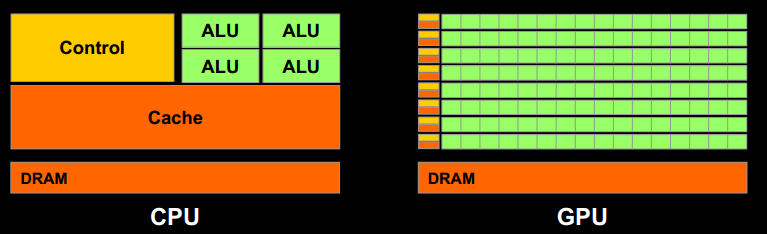
\includegraphics[width=1\textwidth]{figures/GPUCPUimage.png} % trim=4.85cm 15cm 0.85cm 1cm
\caption{A basic representation of the Transistor allocation on a \acrshort{gpu} compared to a \acrshort{cpu}. \citep{NvidiaCUDASeminar}}\label{image:gpucpuimage}
\vspace{-15pt}
\end{figure}

A simple representational comparison of a \acrshort{cpu}'s --- and a \acrshort{gpu}'s transistor usage is shown in \myref{image:gpucpuimage}.
The \acrshort{gpu} consists of many less powerful cores where the \acrshort{cpu} consists of a few more powerful ones, the greater amount of cores allows for more computational power.
But to be able to utilise this computation power a problem must able to be split up, so many or all the cores in the \acrshort{gpu} is used.
As of Q1 2015 an example of a modern high end desktop \acrshort{cpu} is the Intel Haswell core i7 5960X which has 8 cores. \citep{puget}
A contemporary high end \acrshort{gpu} is the NVIDIA GTX 980 which has 2048 CUDA cores. \citep{techpowerup,gtx980}
Due to their architectural differences the \acrshort{gpu} allows for about 12 times more operations per second.\todo{Vi kan sætte en fodnote ind med de beregninger der var her tidligere evt :P ? - Søren}

This makes the \acrshort{gpu} particularly useful for large and complex computations if it is possible to distribute the workload among the \acrshort{gpu}'s cores.
However, the \acrshort{gpu} has an overhead cost.
This means that moving data and computations to the \acrshort{gpu} is time consuming.
Therefore the computation must be of a certain size, before the advantage of parallel \acrshort{gpu} computations exceeds the cost of transferring calculations onto the \acrshort{gpu}.
To illustrate this problem as well as finding an approximate computation size where the \acrshort{gpu} is advantageous some test problems have been written. 
These problems perform different operations on all elements in a matrix. 

\subsection{\acrshort{gpu} and \acrshort{cpu} computations comparison}\label{sub:gpubechmark}
To compare the computational speed of a \acrshort{gpu} and a \acrshort{cpu} for operations on each element in a matrix we have written two programs.
A program written in regular C targeting the \acrshort{cpu} and an equivalent program written in C with CUDA libraries targeting the \acrshort{gpu} for computations.
\todo{Skal der ikke stå noget om hvad CUDA er her ??}
Further explanation of this test and the full source code of both programs and the accompanying scripts can be found in \myref{app:gpuoverhead} and \myref{app:cd}.

Both programs have been run with multiple sizes of the matrix.
The execution times for the two have been compared to find an estimated threshold for when the \acrshort{gpu} power overtakes the data transfer.
The test case for the following comparison consists of seven operations on a square matrix of size n.
As an example, with a square matrix of size $n$ as input the amount of calculations is $7*n^2 = O(n^2)$ operations. 
And there are $n^2 = O(n^2)$ numbers in the matrix which will be operated on.
The operations are division, multiplication, addition and subtraction.
The result can be seen on \myref{image:benchmark}.
\begin{figure}[h!]
\centering
 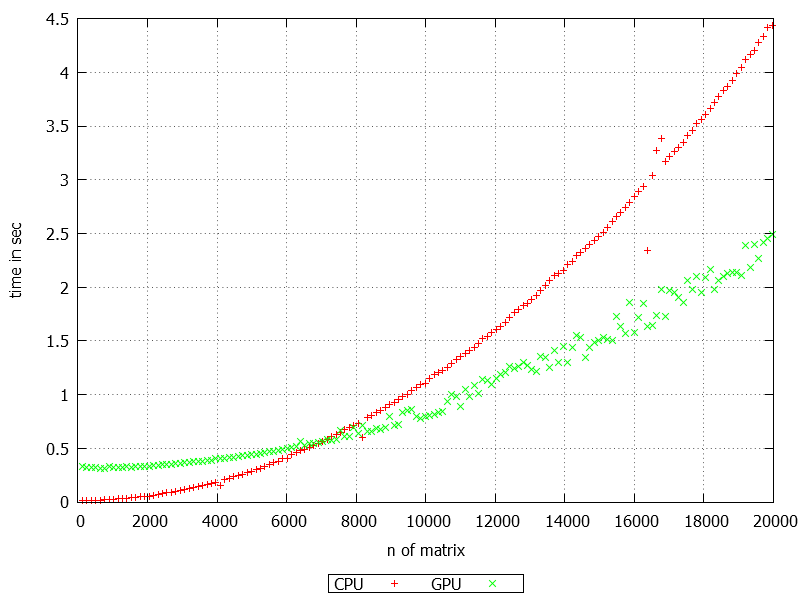
\includegraphics[width=1\textwidth]{figures/benchmark.png} % trim=4.85cm 15cm 0.85cm 1cm
\caption{A benchmark of performing seven operations on each element in a square matrix with size n on a \acrshort{cpu} and a \acrshort{gpu} respectively.}\label{image:benchmark}
\vspace{-15pt}
\end{figure}

The results show that in this case the \acrshort{gpu} becomes advantageous when n reaches about 7000 as can be seen in \myref{image:benchmark}
When n is 7000 the size of the matrix represent operations on almost 50 millions elements.
<<<<<<< HEAD
This is a large amount of data but this is partly due to the simple operations done on the elements in the matrix, we believe that the threshold would happen earlier for a more computation heavy calculation on the elements in the matrix.
=======
This is a large amount of data but this is partly due to the simple operations done on the elements in the matrix, we believe that the threshold would happen earlier for more complex operations on the elements in matrix.\todo{og hvorfra ved vi at det er fordi det er simple operationer? og hvorfor mener vi thresholden ændres med andre operationer?}
>>>>>>> master
In addition to the threshold, the result also confirms that as the dataset grows the \acrshort{gpu} becomes exponentially more useful for computing the data fast.
 %label sec:comparch
\section{Existing solutions} % (fold)
\label{sec:state_of_the_art}
In this section different approaches to \acrshort{gpgpu} using existing programming languages and libraries will be presented.
Each language and library will be running with either the OpenCL or the CUDA framework.
Every language and library described in this section can be found on \myref{tbl:sota} for an overview of their comparisons.
      
\subsection{Libraries} 
There exists libraries for programming languages in order to utilise the \acrshort{gpu} for computations by binding either to OpenCL or CUDA.
Generally the libraries used for \acrshort{gpu} work often requires a lot of boilerplate and has what we deem to be a low level of abstraction.
The level of abstraction is based on how much control the programmer of the code has of the computer's resources.
I.e. if the programmer needs a line of code to allocate memory for each of the computations in the code, that results in low abstraction.
Boilerplate is the pieces of code which will have to be written with little to no alteration, in many different places of the code.
An example could be when making a call to a \acrshort{gpu}, the boilerplate might be the code which handles this communication.
As an example we will look at C, Java and R, and some of their \acrshort{gpu} Libraries.
Jcuda is a library for Java which support the use of CUDA, it has a lot of boilerplate, and low/medium abstraction level. \citep{Java_library}
Jcuda requires many imports and the user needs to allocate a memory block for each element which causes the boilerplate code and the level of abstraction given. \citep{Java_malloc}
C has libraries such as CUDA C, OpenCL C and others.
These C libraries have the same problem as with the Java library as one needs to allocate memory for almost everything, and there is a lot of redundancy which creates a lot of boilerplate.
The abstraction level is therefore deemed low as one must keep in mind what is where and what can be done with each specific element. \citep{C_CUDA} 
There is also different libraries for the R language, one of which is called rpud.
It provides many functions from the R language, which can be performed on the \acrshort{gpu}, and it is based on CUDA.
We deem that it has a high level of abstractions, since it is just function calls, without any memory allocation or direct \acrshort{gpu} calls from the source code. \citep{Rcuda} 

\subsection{Theano (Python)}
Theano is a Python library that allows one to define, optimise, and evaluate mathematical expressions involving multi-dimensional arrays, while utilising the \acrshort{gpu}.
The library has two ways of using the \acrshort{gpu}; one with CUDA as back-end, and the other that should support any OpenCL compatible device as well NVIDIA cards.
The OpenCL implementation however does not support all the options available in the library due to an incomplete port of an old back-end.
While Theano supports CUDA and OpenCL, there is quite a bit of boilerplate and one must write different code in order to use either.	
The scoping rules for Python which Theano uses are quite special where the compiler looks for a variable in four different scopes.
These scoping rules seems to be exclusive to the Python language.
This can cause some problems for new programmers of the language, because these scoping rules are special.
 Theano does not require that the programmer allocates memory for arrays.
We deem that Theano has a medium level of abstraction since one has to declare if the \acrshort{gpu} should be used and can only operate on single precision floats of 32 bits.
But on the other hand Theano does optimise the code by replacing methods with a \acrshort{gpu} versions of the same methods to create transparency. \citep{Theano,Theano_GPU,bergstratheano, LEGB}

\subsection{MATLAB}
MATLAB is a high-level mathematical programming language with an interactive environment.
MATLAB supports the use of parallel computations in the form of using either a \acrshort{gpu} or cloud computing.
It only natively supports the use of CUDA enabled NVIDIA \acrshortpl{gpu} for its parallel computations on \acrshortpl{gpu}, but OpenCL extensions do exist such that it becomes possible to use other devices.
MATLAB uses static scoping  with rules very similar to programming languages like.
The user of MATLAB much declare when the \acrshort{gpu} must be used and also allocate memory for these tasks.
Declaring the memory gives a lot of boilerplate since it needs to be done for each element that one wants to compute. \citep{MATLAB_backend,MATLAB_benchmark}

Using the interactive environment provided by MATLAB there are built in tools for parallel computations on \acrshortpl{gpu}.
These tools provide a higher level of abstraction such as parallel for-loops (parfor) and special array types for distributed processing.
For \acrshort{gpu} computing MATLAB simplify parallel code development by abstracting away the complexity of managing computations and data. \citep{MATLAB_parallel}

\subsection{Julia}
Julia is a high-level, high-performance dynamic programming language for technical computing, with syntax familiar to users of other technical computing environments.
Julia is designed for parallelism and cloud computing; making it efficient and easy to use for these tasks.
Julia has a high level of abstraction because the user only needs a single keyword (\@parallel) for it to do the calculation in parallel.
The code is therefore looking clean without any boilerplate and is easy to read.
Julia uses both OpenCL and CUDA as back-end making it very compatible and easy to use on different systems and devices.
Julia uses similar scoping rules as MATLAB.\citep{Julia_Git, Julia_scope,Julia}

\begin{table}
	\centering
    \colorlet{shadecolor}{gray!40}
    \rowcolors{1}{white}{shadecolor}
	\begin{tabular}{|l|c|c|l|l|}
	\hline
	\textbf{Language} & \textbf{CUDA}         & \textbf{OpenCL} & \textbf{Abstraction} & \textbf{Comment}			  		\\ \hline
	Theano   & \cmark           & \cmark            & High      &  Native                                                          \\ \hline
	Matlab   & \cmark           & \cmark            & Low/High        &  OpenCL via extensions, CUDA is native                                                         \\ \hline
	Julia    & \cmark           & \cmark              & High        &  Both via extensions                                                          \\ \hline
	R        & \cmark           & \cmark            & Low/High    & Abstraction is depended on the use of either CUDA or OpenCL \\ \hline
	C   & \cmark           & \cmark            & Low         & via CUDA C, and OpenCL C (Both are supersets of C)                                           \\ \hline
	Java     & \cmark           & \cmark              &   Low          & Bindings such as jcuda and jocl                                            \\ \hline
	\end{tabular}
	\caption{Existing GPU supporting languages. }\label{tbl:sota}
\end{table}
                

\subsection{Conclusion}  

The different languages mentioned in this section all have some way of communicating with the \acrshort{gpu} using both CUDA and OpenCL, which also can be seen on \myref{tbl:sota}.
They all require the user to specify when to use the \acrshort{gpu} instead of the CPU, and the level of abstraction varies, where some require a lot of control of the programmer, and others require specific function calls to \acrshort{gpu} functions.

This explicit processor targeting seems inconvenient, and it takes away focus from the calculations done in the program.
On the other hand, it gives the programmer more control of where the code is executed.
This aspect requires a deeper knowledge of processor architecture, and we deem that greater abstraction is more important than the control of processor targeting.

They are all usable for general purpose programming, except the libraries for R, which only provides the programmer with specific R functions to be computed on the \acrshort{gpu}.
For scientific computing, especially oriented towards matrices and vector calculations such as linear algebra uses, these are all viable options.

The control of memory on the CPU and the \acrshort{gpu} is different, so allocating memory is more difficult when you transfer the calculations to the \acrshort{gpu}.
Therefore languages that require the programmer to allocate memory themselves, takes away focus from the computations that need to be done.
We deem that allocating memory for arrays and matrices is unnecessary.
                     
\newpage
\section{Problem statement}
\label{sec:problem}

\myref{subsec:gputest} shows that calculations on matrices, when sufficiently large, can take a long time to compute sequentially. 
Therefore it is smarter to parallelise these computations, and even better to do so on a \acrshort{gpu} compared to a \acrshort{cpu}, due to its internal architecture.
Many linear algebra calculations can be parallelised since it often contains large datasets where operations on the data does not depend on previous calculations.
An example of this could be matrix calculations where most operations can be split into independent sub calculations.
Therefore the computation time of these calculations can be significantly improved using the parallel computing capabilities on the \acrshort{gpu}, given the matrices are of sufficient size.

Writing programs which can be run on a \acrshort{gpu}, can be time consuming using the languages found in \myref{sec:state_of_the_art}.
It is time consuming due to the difficulty of writing code in some of these languages like OpenCL C, and CUDA C.
Therefore we believe that more abstraction and less boilerplate when writing code to the \acrshort{gpu} would serve well and reduce the workload on the people programming for the \acrshort{gpu}.
In the rest of this paper, the following problem will be thoroughly investigated, not only in the design of the syntax and the semantics of the language, but also in the design of the compiler.\todo{Vi beslutter os allerede her for at lave en compiler? Skal vi ikke fjerne det og ændre det til noget med "the design of translating the code" eller noget? -Søren}

\[
  \left[
  \begin{minipage}{\textwidth}
  \centering
  \begin{minipage}{0.96\textwidth}
  How does one design a programming language, with a corresponding compiler, which compiles source code to execute on the \acrshort{gpu} at runtime for certain linear algebra calculations, such as matrix operations?
  %%How does one design a programming language, with a corresponding compiler, for technical computing that is capable of performing common operations of linear algebra, while targeting \acrshort{gpu}s as execution platform?
  
  %%Alternative%%
  %%How do you design a programming language and a compiler for this language, which is able to compute parallel linear algebra calculations using the \acrshort{gpu} instead of the CPU without the programmer specifying so?
  
  %%How would a programming language and a compiler be programmed for a language specific for computing paralles linear algebra calculations using the \acrshort{gpu} instead of the CPU without the programmer choosing so specifically.  

  %%Is it possible to design a programming language for numerical computation with a focus on matrices, which is simple to use but also fast by taking advantage of the \acrshort{gpu} on modern computers? How would such a language be implemented? 

  %%How can a simple programming language, which compiles code targeting the \acrshort{gpu}, be construed so it's easier to perform matrix calculations? 

  %%Is it possible to construct a programming language in which matrix operations and linear algebra can be performed, with the power of the \acrshort{gpu}, without the programmer having to worry about boilerplate code. 
  \end{minipage}
  \end{minipage}
    \right]
\]
\chapter{Methodology}\label{chap:methdology}

This chapter will briefly explain the development method we will use to organise our work to find an answer to our problem statement. 
Inventing a programming language and developing a compiler for it, is a complex and time consuming process, so having a method for the development helps, which is why our methodology is discussed in this paper.

\section{Development Method}
In order to develop a language and its compiler, a comprehensive understanding of how programming languages work, and how compilers are structured is required.
Therefore we need to use the tools taught in the courses of this semester.
As these tools are acquired over a period of time the planning and development of a language cannot be done beforehand; with this in mind,, it makes sense to use an iterative development process.
One such method is Scrum, which group members have had success with on previous semesters.
Therefore we choose to develop this project using an adaptation Scrum.
In our adaptation we will make use of Scrums organisational tool, such as the Scrum board, daily Scrums and sprints.

The Scrum board brings an overview of active subproblems to be solved for the project.
To solve these the daily Scrums are used to partition workloads to each member of the project as well as acknowledge potential issues.
The sprints keeps the development iterative which in turn allows us to use newfound knowledge that we may not have had in previous sprints.
We will not have the specific roles which you would normally find in Scrum, such as the Scrum master or the product owner. \citep{Scrum}
The reason for this is, partly due to development methods not being in the curriculum for this project, but also due to the project not having use of these tools.
There is no customer for whom we are developing the compiler nor is there really time for one person in the group to be Scrum master, as he would still need to focus a lot on the tasks the rest of the group are also partaking in.
With this method we are able to work in short sprints of one to two weeks, which gives us the opportunity to incorporate the tools, concepts, and methods we learn during the development process.

We have a hard deadline to take into account, which forces us to have a certain number of sprints, instead of being able to develop on the project eternally.
That is not to say we do not plan ahead, but our long term plans are versatile, i.e. if we learn of something new, it is easier for us to implement this new knowledge in our project by going back to fix mistakes and adding features, compared to if we used linear development method.

% ALTERNATIVE?!!?
%\section{Development Method}
%We have decided to use parts of the agile development method Scrum. 
%Our development method is not Scrum but iterative with parts of Scrum to organise group work. 
%The parts of Scrum which we are using is the Scrum board, daily Scrum and sprints with user stories. 
%This is to make communication, organisation, and teamwork easier. 
%\gls{gamble} is used to refer to our languange   
\chapter{Language Criteria} % (fold)
\label{cha:language_criteria}
>>>>>>> master:chapters/Criteria.tex
When evaluating programming languages one must first agree on the goals of a given language's characteristics.
Robert W. Sebesta has given some criteria which can be evaluated from, we will use these criteria to design our language and to state which criteria are important to the language we are designing.\citep{Sebesta}
The criteria can be seen on \myref{tbl:concepts}.
First a brief description of the criteria will be given, followed by how we rate these criteria for our language according to the information found in \myref{cha:introduction}.
\begin{table}[h]
	\centering
	\colorlet{shadecolor}{gray!40}
    \rowcolors{1}{white}{shadecolor}
	\begin{tabular}{|l|c|c|c|}
	\hline
	\textbf{Language Concepts} & \textbf{Readability}  & \textbf{Writability} & \textbf{Reliability}   \\ \hline
	Simplicity                 & x      		       & x             		  & x           		   \\ \hline
	Orthogonality              & x 				       & x             		  & x           		   \\ \hline
	Data types                 & x 				       & x             		  & x           		   \\ \hline
	Syntax design              & x 				       & x             		  & x           		   \\ \hline
	Support for abstraction    &                       & x             		  & x           		   \\ \hline
	Expressivity               &                       & x             		  & x           		   \\ \hline
	Type checking              &                       &               		  & x           		   \\ \hline
	Exception handling         &                       &               		  & x           		   \\ \hline
	Restricted aliasing        &                       &               		  & x           		   \\ \hline
	\end{tabular}
	\caption{Language evaluation criteria and the characteristics that affect them.}\label{tbl:concepts}
\end{table}

We want it to be easy for programmers and mathematicians alike to write and read programs in our language.
The focus should be on calculating the problem at hand, without having to conform to low level language specifics, controlling memory etc.
Our language must adhere to the concept of simplicity, which means that the number of basic constructs is kept low. 
This results in high levels of both readability and writability as can be seen on \myref{tbl:concepts}.
The language supports abstraction over the programmer's hardware, by not having to specify where the computations must be run, or having to allocate memory.

To get an idea of what each criterion expressed, we will in the following text, describe our thoughts and goals in respect to the several of the  concepts in \myref{tbl:concepts} deemed important to \gls{gamble}.
Simplicity is important in the language of \gls{gamble}.
It is so because of the goals stated in \myref{sec:problem} and based on the other languages examined in \myref{sec:state_of_the_art}, simplicity is important when designing a language where the focus lies in writing code fast and easy, which can take advantage of the \acrshort{gpu}.
It is so because this goal does not require a large language.
Syntax design is also deemed an important criterion, it is so because the language should be familiar and easy to learn for beth experienced but especially newer programmers.
Data types is another important criterion for \gls{gamble}, as stated in \myref{sec:problem} the language should be able to handle a matrix data structure and furthermore is at stated in the problem statement should the language utilise the \acrshort{gpu} without the programmer specifically stating it, in that respect a high level of abstraction is important too. 

Based on the earlier discussions, exception handling is seen as a way of making the language more complex, therefore a goal in \gls{gamble} is to catch errors like type mismatch on compile time, which strongly eliminates the need for exception handling.


\section{Success criteria}\label{sec:OurCriterias}
We deem our language and compiler to be a good solution for our problem statement if it upholds to the following criteria:

\begin{itemize}
	\item Calculating matrix and vector calculations on the GPU, without the programmer specifically specifying it to do so.
	\item Can implicitly calculate matrix operations on the \acrshort{gpu} faster than regular C being run on the \acrshort{cpu}, when sufficient large matrices are provided.
	\item Expresses a high level of read- and writability, by adhering to the concept of simplicity and having a familiar syntax design.
	\item Provides reliability, with type and scope checking.
	\item Gives descriptive and fulfilling error messages, for easier debugging, resulting in better writability.
\end{itemize}

A more precise description of \gls{gamble}'s design principles abiding to Sebesta's criteria will be presented and argued for in the following chapter.
% chapter language_criteria (end)                   
\chapter{Language Design}
\label{cha:Design}
%Metatext for design chapter
In this chapter the design of the language called \gls{gamble} will be presented.\todo{Hvad står Gamble for?}
First with a brief description of our design philosophy for \gls{gamble} will be introduced to clarify what this language is attempting to achieve and why.
The design philosophy will address some of the criterias found in \myref{sec:OurCriterias}.
Furthermore the features and design of \gls{gamble} will be documented later in this chapter.

%\gls{gamble} is used to refer to our languange
\section{Design Philosophy}\label{sec:phil}

The focus for \gls{gamble} is to use the computational powers of the \acrshort{gpu} to handle such computations without it being inconvenient for the programmer.
As described in \myref{sec:state_of_the_art} several libraries and languages allows the programmer to explicitly designate workloads to the \acrshort{gpu} however this often requires explicit memory handling as well.
Keeping the rules and syntax of \gls{gamble} familiar to other languages makes it more accessible and reduces the time required for users to familiarize themselves with it.
This is done by using a C-like syntax, while stripping \gls{gamble} of features we deem not necessary for a language which main focus lies in using the \acrshort{gpu} for  linear algebra calculations.
The C-like syntax is chosen because the top 5 languages on Tiobe's list of most popular programming languages are C-like, and therefore if \gls{gamble} resembles these languages, it will be more familiar to start programming in \gls{gamble} which in turn makes it easier to implement ones algorithms.\citep{TIOBE}
As the \acrshort{gpu} is the resource being used to achieve more computational power, the data computed must also be applicable to the niche of the GPU, i.e. the data must be parallelisable as explained in \myref{sec:comparch}.
This basic need will influence how data is represented, and also put focus onto matrices and vector calculations, which as mentioned before can often be parallelised.

\textbf{Allow the programmer to use the \acrshort{gpu} without it being inconvenient}

Due to \gls{gamble} being focused on numerical computations, allowing the programmer to focus on managing the mathematical aspects is the main focus.
Therefore having the programmer control the runtime architecture seems an unnecessary distraction.
\gls{gamble} takes care of designating the computations to the best suited processing unit, whether it be the \acrshort{gpu} or the \acrshort{cpu}, as such any inconvenience in that process is removed from the programmer whose focus can be solely on the mathematics.
This abstraction therefore results in better writability.

\info[inline]{Maybe we should add automatic memory management here, it is *HARD* in OpenCL, CUDA etc. so it would make a nice point? -- Troels}

\textbf{Avoid implementing unnecessary data types and features}

As the purpose of \gls{gamble} is to use the \acrshort{gpu} for calculations which can be parallelised implementing features or data types, that do not hold any regard to this aspect would clutter the language.
Additionally \gls{gamble} should not try to adapt itself towards purposes for which it is not designed, an example of excluding such features is the fact that strings are not part of the language, this choice and others like it are further documented later in this chapter.
This makes \gls{gamble} simpler, and therefore both easier to read and write.
\todo{Denne udtalelse gør at vi nok bør lytte til Thomas og helt slette afsnit 14.6 om general purpose Gamble.. - Søren}

\textbf{Let the language be somewhat familiar to read and use}

As mentioned the main purpose of \gls{gamble} is to use the \acrshort{gpu} for computations, and is focused on doing computations, not developing new software.
As such \gls{gamble} would most often be used where this niche is required.
It may even be likely that it is not used when developing an algorithm to do computations, but first used once the algorithm is to be implemented during the algorithm design process, and can then be applied to bigger sets of data.\citep{AlgorithmDesign}
This is because of the large overhead as explained in \myref{sec:comparch}, it will be faster to perform a test of an algorithm with smaller datasets in other languages, like C.
Therefore to use the niche that \gls{gamble} proclaims, having the language be familiar makes it easier to use for its pure computational aspect, and improves on \gls{gamble}'s read- and writability.

In the following sections different parts of \gls{gamble} will be investigated.

\section{Core syntax choices}
The source code must be encoded in UTF-8, but only the ASCII alphabet and numbers are allowed for identifiers and values, this is to simplify the parsing. 
The language is case sensitive, because the most used languages seen on TIOBEs index\citep{TIOBE} are also case sensitive.
When a language is case sensitive it is possible for the programmer to name different parts of the code like he pleases, resulting in higher readability.
Some languages, such as Python, uses whitespace and indentation to indicate scope, in our language scope is indicated by curly brackets like many existing languages\texttt{\{\}}.  

\subsection*{Comments}
It is useful to be able to write comments in code to annotate the meaning of some code.
If a language were not to have the possibility to write comments, then the source code could be hard to understand.
Source code without comments might be difficult to return to after some time away from it, since the programmer would have to reread the entire code, instead of a few good comments.\citep{Commenting}
Therefore both single line and multi line comments can be used in \gls{gamble}. 
``//'' is used for single line comments, meaning that everything after the ``//'' until the next newline is ignored by the compiler, also known as C++ style comments. 
``/* */'' is used for multi line comments, meaning that everything between ``/*'' and ``*/'' is ignored by the compiler, also known as C style comments. 

\subsection*{End of statement terminator}
When choosing an end of state terminator there are two main choices.
The newline character as a terminator or another symbol, often semicolon (;).
The use of newline is often used in simple languages e.g. MATLAB or other mathematical oriented languages. 
We deem the main value of using the newline are simplicity and a decrease in errors due to forgotten semicolons.
Semicolon is as mentioned the other main choice, this choice has been used through many programming languages throughout the history. 
The main advantage of a end of statement terminator  like semicolon is that it allows freeform code. 
This freeform allows to have multiple statements in one line or allows long statements to span across multiple lines.
We deem this to enhance the readability of the code.
Furthermore the semicolon terminator allows for a simpler syntax and compiler design.
As mentioned before forgotten semicolons can result in compiler errors, we deem this as the biggest disadvantages of this end of statement terminator.

Based on this analysis we have chosen to use the semicolon as end of statement terminator, for easier parsing.

\subsection*{Scope}\label{subsec:Scope}
If a programming language contain no implementation of scoping rules, then one must assume that all the source code in a given program would be in the same scope.
Such a single scope would mean that any variable can be used form any place in the code. 
Mostly, as briefly described in \myref{sec:state_of_the_art}, a programming language implements some kind of scoping rules.
There are several reasons for this, the main reason being it gives the programmer more control of the code and reduces the chance of changing variables by accident.
There exist two main methods of scoping, static and dynamic scoping.
As seen in \myref{sec:state_of_the_art} most of the languages examined in this section used a form of static scope. 
\gls{gamble} will use this form of scoping because we find it to be the easiest to work with and less prone to errors than dynamic scoping.
The scope rules of \gls{gamble} are as follows:

A variable is in scope from its declaration until the end of the block it is declared in.
An inner block such as a control flow structure, see \myref{subsec:control-flow} for more, has access to the variables from the outer scope. 
It is also not allowed to redeclare a variable which is already declared in the current scope. 
Additionally any function is in scope of any other function including itself, this also allows recursion. 
- This is static scoping without information hiding. 

\subsection*{Structure}\label{subsec:Struc}
The structure of the source code to a \gls{gamble} program is shown in \myref{lst:Structure}.
For a high level of readability we have decided  to split the source code up in segments.
A single segment contains only a small part of source code.
Including of other files are, like in many other languages, written in the top segment, this is to make it easy to get an overview of any and all included libraries. 
All function declarations are written in the next segment followed by the main statements which is the last segment.
This collects the main statements, which makes it easier for a programmer to get an overview over the order of execution, compared to if the main statements were allowed between the function declarations.
This sectioning also makes it easier to write a context free grammar for the language.

\begin{lstlisting}[caption={Source code file layout in \gls{gamble}},frame=tlrb,label={lst:Structure}, numbers=none]
Libary inclusions

Function declarations

Statements
\end{lstlisting}

\section{Types and Variables} \label{sec:Types}
%http://www.informit.com/articles/article.aspx?p=2103809&seqNum=3
\gls{gamble} uses three primitive data types; integers (int), floating points (float) and boolean values (bool), as well as two composite data types; matrices and vector. 
In \gls{gamble} any variable must be initialised when it is declared. 
This avoids any null reference which can cause runtime errors in many languages such as C, C\# and Java.
In \gls{gamble} all variables are statically stored, there are several reasons for this and therefore the language does not implement neither explicit or dynamic memory handling.
The first reason for this is that the purpose of the language is to perform arithmetic operations on the \acrshort{gpu}, so by excluding this the language's simplicity increases, and therefore its read- and writability increases.
A second reason being that the size of every variable in \gls{gamble} is unchangeable.
Any vector and matrix will be allocated on the heap by the compiler.
Manual memory handling could increase the number of possible programs in the language and is therefore seen as a viable extension to future versions of \gls{gamble}.


\subsection*{Integers and floating points}
An integer is a whole number either positive or negative, represented by the two's compliment method. 
Meaning that it ranges from $-(2^{n-1}) $ to $2^{n-1} - 1 $, where n is the number of bits used.
A floating point number is an approximation to a real number. 
It is separated in 3 parts, the sign bit, the mantissa and the exponent. 
Floats in \gls{gamble} are in base 2, the value of a float is calculated by $ (-1)^{sign bit} \cdot mantissa \cdot 2^{exponent} $. 
Integers and floating point numbers default to 32 bits with the keywords \texttt{int} and \texttt{float}. 
It is possible to declare 16 and 64 bit integers and floating point numbers by postfixing their size to their respective keywords, e.g. \texttt{float64} or \texttt{int16}. 
It is useful to be able to specify the size of an integer or a floating point number, as data transfer can cause a lot of overhead particularly when transferring data to and from the \acrshort{gpu}. 

\subsection*{Boolean}
A boolean value is either true or false. 
These are used for control structures in \gls{gamble} which takes a boolean value as a parameter. 
But can also be used for any means which the programmer finds useful. 

\subsection*{Vectors and Matrices}
A vector in \gls{gamble} is a sequence of entries which are each the same primitive data type. 
The dimension of a vector is immutable, meaning that its dimension cannot be changed after its declaration. 
A matrix is multiple row vectors inside a column vector, each row vector is the same dimension. 
As for other variables both vectors and matrices must be initialised when they are declared. 
This is done with the syntax shown in \myref{lst:matrix}.
Here it is also seen why the use of ``;'' is a smart choice for ending statements.

\begin{lstlisting}[caption={Creating a matrix},label={lst:matrix},numbers=none]
matrix<int> m = [1, 0; 
                 0, 1];

rowvector<int> rv = [1, 0];
\end{lstlisting}

\subsection*{Operators}
Available operators in the language can be found on \myref{tbl:operators} with a short description.  
It is not possible to use operators with matrices or vectors, functions which support different operations on these types will be included in a library.
\begin{table}[h]
    \centering
    \colorlet{shadecolor}{gray!40}
    \rowcolors{1}{white}{shadecolor}
    \begin{tabular}{|c|l|l|l|l|l|}
    \hline
    \textbf{Operator}  & \textbf{Integer}                   & \textbf{Floating point number}    & \textbf{Boolean}      & \textbf{Matrix}       & \textbf{Vector}     \\ \hline
    +                  & Addition (infix)                   & Addition (infix)                  & Type error            & Addition (infix)      & Addition (infix) \\ \hline 
    -                  & Subtraction (infix)                & Subtraction (infix)               & Type error            & Subtraction (infix)   & Subtraction (infix) \\ \hline 
    ++                 & Increment (unary,pre-, postfix)    & Increment(unary,pre-, postfix)    & Type error            & Type error            & Type error \\ \hline    
    --                 & Decrement (unary,pre-, postfix)    & Decrement(unary,pre-, postfix)    & Type error            & Type error            & Type error \\ \hline
    *                  & Multiplication (infix)             & Multiplication(infix)             & Type error            & Type error            & Type error      \\ \hline
    \%                 & Remainder (infix)                  & Modulo(infix)                     & Type error            & Type error            & Type error  \\ \hline
    /                  & Division (infix)                   & Division (infix)                  & Type error            & Type error            & Type error \\ \hline
    \&\&               & Type error                         & Type error                        & Logical and (infix)   & Type error            & Type error \\ \hline 
    ||                 & Type error                         & Type error                        & Logical or (infix)    & Type error            & Type error \\ \hline 
    ==                 & Equality (infix)                   & Equality* (infix)                 & Type error            & Type error            & Type error \\ \hline 
    !=                 & Inequality (infix)                 & Inequality* (infix)               & Type error            & Type error            & Type error \\ \hline
    <=                 & Less than or equal to (infix)      & Less than or equal to* (infix)    & Type error            & Type error            & Type error \\ \hline
    >=                 & More than or equal to (infix)      & More than or equal to* (infix)    & Type error            & Type error            & Type error \\ \hline
    <                  & Less than (infix)                  & Less than (infix)                 & Type error            & Type error            & Type error \\ \hline
    >                  & More than (infix)                  & More than (infix)                 & Type error            & Type error            & Type error\\ \hline
    \end{tabular}
    \caption[List of operators on primitive data types in GAMBLE.]{List of operators on primitive data types in GAMBLE.\@*Equality comparisons on floating point number may be incorrect.}\label{tbl:operators}
\end{table}
\vspace{-20pt}

%\subsection*{Memory handling}
%Locally declared and small and simple variables will be written to the stack, while large quantities of data must be written to the heap. 
%To manage the heap in a programming language one must decide how the management must be implemented.
%At the topmost level there exist to different approaches, the first being explicit memory handling as seen in C with function calls like \texttt{alloc()} and \texttt{free()}. 
%The second approach is dynamic memory handling, often called garbage collection.
%While  manual memory handling is a very low level concept, it has some advantages over dynamic memory handling, for instance manual handling gives the users full control over a programs resources and while this can be hard o get right, can both increase the simplicity of the compiler and increase a programs runtime execution speed because garbage collection can be a complex runtime process.\citep{Sebesta, gribble}

\section{Functions}
\todo{Forklar print funktionen}
Functions are blocks of code which can be called to do a specific computation, often but not always, a function takes some variables as inputs.

This section will describe \gls{gamble}'s use of functions. 
Like in many other languages it is possible to declare your own functions in \gls{gamble}.
This is useful for organising code, and reusing parts of the source code.
Functions in \gls{gamble} can take input, but are not required to, the inputs can be any of the types the languages support.
Because of high implementation cost in the compiler, it is not possible to use a function as an input for a function.


\subsection*{Function identifiers}
When declaring a \gls{gamble} function it is required to write the body of the function immediately after.
This is to avoid lookahead which function prototypes in C requires.
A function identifier is exactly like C, with the \texttt{return type} then the \texttt{functionname}, \texttt{(formal parameters)} and finally the \texttt{\{body\}}.
The function body can contain a number of statements and various control flows.
Furthermore it can contain calls to other functions or calls to the function itself, and hereby recursion is a possibility in \gls{gamble}
An example of a function identifier can be seen on \myref{lst:functionID}.
Other syntaxes could have been used, but not only is this the way C does it, it is also widely used in many other languages i.e. C\# and Java.

\begin{lstlisting}[caption={Function Identifier},label={lst:functionID},numbers=none]                                                        
int add(int a, int b)
{
    return a + b;
}
\end{lstlisting}

\subsection*{Function calls}
After a function has been declared it can be called. 
A function call contains the identifier and parameters for the function. 
The syntax in \gls{gamble} is the same as in many other programming language and shown in \myref{lst:functionCall}. 

\begin{lstlisting}[caption={A function call in \gls{gamble}},label={lst:functionCall},numbers=none]
add(4, 3);
\end{lstlisting}


\subsection*{Return value}
Functions have a return value which can be seen on \myref{lst:functionID}.
The return values are all the types in \gls{gamble} mentioned in \myref{sec:Types} and void. 
A void function will not return anything, but instead can be seen as a procedure.
This choice was made because \gls{gamble} should be able to return all the different types in the language from a function, but also be able to perform these procedures which a void function may do.
The value or type to be returned is preceded by the keyword \texttt{return}, just like it is in C and other C-like languages.
An example can be seen on \myref{lst:returnFunction}.

\begin{lstlisting}[caption={Return Function},label={lst:returnFunction}]
int a = 0;

a = add(4, 3);
\end{lstlisting}


\subsection*{Print function}\todo{rename maybe}
In \gls{gamble} we have one function that is ready-made. It is a print function.
The function is special because it can both take variables, numerical values and strings as input parameter.
Since string is not a valid data type in \gls{gamble} this function is special. 
With the print function it is possible to give the user a visual representation of the computations result, in the console.
A simple print function which take string inputs increases both readability and writability.
Strings in the print function allows the programmer to write easier understandable and readable program output. 
%STD LIB EVT?!
\section{Control Flow}\label{subsec:control-flow}\todo{Troels: Imo er hele dette afsnit på en måde for langt. }
Control flow is any part of the language in which a branch occurs. 
A branch is in this case a change in which instruction happens next. 
These come in three variations: primitives, choice and loops.
C, C\#, Java etc. contain some or all of these elements to control the flow of a program:

\textbf{Primitive:}
\begin{itemize}[noitemsep,topsep=-5pt] %removes whitespace before and between points.
    \item \texttt{goto}
\end{itemize}

\textbf{Choice:}
\begin{itemize}[noitemsep,topsep=-5pt] %removes whitespace before and between points.
    \item \texttt{if/if-else}
    \item \texttt{?:} (Ternary operator)
    \item \texttt{switch}
\end{itemize}

\textbf{Loops:}
\begin{itemize}[noitemsep,topsep=-5pt] %removes whitespace before and between points.
    \item \texttt{while}
    \item \texttt{for}
    \item \texttt{foreach}
    \item \texttt{do..while}
\end{itemize}

If a programming language has if, goto and label then the other constructs can be made.
For example a while-loop can be translated to a combination of the if and goto statements, this is shown in \myref{ifgotowhile1} and \myref{ifgotowhile2} written in C. 

\noindent\begin{minipage}{.45\textwidth}
\begin{lstlisting}[caption=Loop made with while.,frame=tlrb, label=ifgotowhile1, numbers=none]{Name}
while ( condition )
{
    statement();
}
\end{lstlisting}
\end{minipage}\hfill
\begin{minipage}{.45\textwidth}
\begin{lstlisting}[caption=The same loop with if and goto.,frame=tlrb, label=ifgotowhile2, numbers=none]{Name}
label startOfLoop:
if ( condition )
{
    statement();
    goto startOfLoop;
}
\end{lstlisting}
\end{minipage}

The same can be done with the \texttt{for} and \texttt{do..while} loops. 
This means that the only need control structures should be \texttt{if} and \texttt{goto}. 
However the use of goto is considered harmful, because it is easy to make mistakes when using it. \citep{DijkstraGoto}
Even though \texttt{for} and \texttt{while} are similar, they are often used in different contexts.
The for loop is useful for iterating over a collection or knowing exactly how many time the code is executed. 
Therefore we have decided to include both \texttt{for} and \texttt{while} in \gls{gamble}, but not \texttt{foreach} and \texttt{do..while}, this is to simplify the number of control structures.

We have decided to keep the traditional \texttt{if} and \texttt{if-else} constructs. 
These are useful, and can achieve the same as a \texttt{switch}, by chaining if-else statements, so we have excluded the switch construct. 
The ternary operator, also known as the inline if, written as \texttt{?:} in C and many other languages, is useful for compacting code to make it more readable, therefore we include it in \gls{gamble}.

\subsection{if, if-else and ?:} \todo{Jeg blander meget rundt i statement og construct, kan ikke helt beslutte mig. }
Examples of if/if-else \gls{gamble} are shown in \myref{iflst} and \myref{ifelselst}. 
The condition is enclosed in a parenthesis this is to make the if construct similar to the function call, in which the parameters are in a parenthesis. 
All the conditional code must be enclosed in a curly bracket, this is to make the code more readable. 
The use of curly brackets is to make them similar to functions to make the language more alike \todo{mangler et godt fagord her. marc: more familiar/relateable/orthogonal?}.

\noindent\begin{minipage}{.45\textwidth}
\begin{lstlisting}[caption=An if statement in \gls{gamble}.,frame=tlrb, label=iflst, numbers=none]{Name}
if ( condition )
{
    statement();
}
\end{lstlisting}
\begin{lstlisting}[caption=A use of \texttt{?:} in \gls{gamble}.,frame=tlrb, label=terlst, numbers=none]{Name}
condition ? ifTrue() : ifFalse();
\end{lstlisting}

\end{minipage}\hfill
\begin{minipage}{.45\textwidth}
\begin{lstlisting}[caption=An if-else statement in \gls{gamble}.,frame=tlrb, label=ifelselst, numbers=none]{Name}
if ( condition )
{
    statement();
} else {
    alternative_statement();
}
\end{lstlisting}
\end{minipage}

An example of the ternary operator \texttt{?:} is shown in \myref{terlst}. 
If the boolean statement before the question mark is true, then the first statement is executed otherwise the second is. 
The ternary operator can also be used for an assignment, only if the value getting assigned to is left of the question mark.
As the ternary operator allows any statement in its middle body, it is possible to chain them together, just like a if-else chain. 

\subsection{while}
An example of the while loop in \gls{gamble} is shown in \myref{whilelst}. 
The syntax is identical to the if statement, which also makes it look like a function in certain ways. 
It's also identical to the syntax found in many other programming languages and is therefore similar to many programmers. \todo{Skal sådan et argument være med?}

\noindent\begin{minipage}{.40\textwidth}
\begin{lstlisting}[caption=A while loop in \gls{gamble}.,frame=tlrb, label=whilelst, numbers=none]{Name}
while ( condition )
{
    statement();
}
\end{lstlisting}
\end{minipage}\hfill
\begin{minipage}{.50\textwidth}
\begin{lstlisting}[caption=A for loop in \gls{gamble}.,frame=tlrb, label=forlst, numbers=none, language=C]{Name}
for ( initialize; condition; update )
{
    statement();
}
\end{lstlisting}
\end{minipage}

\subsection{for}
An example of the for loop in \gls{gamble} is shown in \myref{forlst}.
An alternative to this syntax is one which allows an iteration over a collection such as a foreach or one that iterates over a range.
Examples of how such a syntax should be is shown in \myref{forextlst}.

\begin{lstlisting}[caption=Alternative syntaxes for the for loop.,frame=tlrb, label=forextlst, numbers=none, language=C]{Name}
// iterates over every int in the range.
for ( int i in range 0:10 )
{
    statement(i);
}
// iterates over every other int in the range.
for ( int i in range 0:10:2 )
{
    statement(i);
}
// iterates over each element as a reference to the element in the collection
foreach ( item i in collection )
{
    statement(i);
}
// iterates over each index in a collection
foreach ( index i in collection )
{
    statement(collection[i]);
}
\end{lstlisting}

These each have the strength of expressing clearly what they do, however they are easily expressed in the form expressed in \myref{forlst}.

\section{Reserved Words}
% (fold)
\label{sec:reserved_words}
In \gls{gamble} there exists a number of reserved words used for types and language constructs among others.
These reserved words, also known as language keywords, cannot be used as identifiers in the language. 
However, not all keywords are reserved words.
This is because keywords such as \texttt{if} and \texttt{for} are often followed by a specific construct.
In fact most cases of keyword usage require some sort of special construct, hereby rendering the keyword unambiguous.\todo{Det ved vi vist ikke hvad er på det her tidspunkt?  - Søren, Nu er unambigious jo ikke noget fagterm så det kan vi sagtens bruge - Marc | enig med Marcus - msm}
As an example, this makes it possible to use \texttt{if}, along with all other keywords, as identifiers in FORTRAN, but this is not the case in \gls{gamble}. \citep{fortran_identifiers}
Keywords in \gls{gamble} are considered reserved, because it minimises the lookahead needed, and therefore simplifying the lexing process while also increasing readability.\todo{Man ved ikke hvad en lexer er på dette tidspunkt. - Corlin}
All the reserved words of \gls{gamble} can be seen in \myref{res:words}.
\begin{table}[h!]
	\centering
	\def\arraystretch{1.5} \setlength{\tabcolsep}{2em}
	\begin{tabular}{l l l l l}
        \texttt{int}     & \texttt{int16}     & \texttt{int32}     & \texttt{int64}     & \texttt{bool}    \\
        \texttt{float}   & \texttt{float16}   & \texttt{float32}   & \texttt{float64}   & \texttt{void}    \\
        \texttt{matrix}  & \texttt{vector}    & \texttt{true}      & \texttt{false}     & \texttt{fileToMatrix} \\
        \texttt{if}      & \texttt{else}      & \texttt{for}       & \texttt{while}     & \texttt{matrixToFile} \\
        \texttt{print}   & \texttt{rows}      & \texttt{cols}      & \texttt{return}    & \texttt{include} \\
    \end{tabular}
    \caption{Reserved words of \gls{gamble}}\label{res:words}
	\def\arraystretch{1}
\end{table}

Besides the reserved words \gls{gamble} contains literals, which also cannot be used as identifiers.
The literals in \gls{gamble} are \texttt{true} and \texttt{false}.\todo{Er tal ikke også literals :p ?}
If \gls{gamble} were to provide a \texttt{null} value, this would be a literal as well.

% section reserved_words (end)

\chapter{Syntax}\label{chap:syntax}

To describe the formal syntax of \gls{gamble}, and to parse the language, it is necessary to write a \acrfull{cfg}.
This chapter will explain what a \acrshort{cfg} is, and the problems of creating one.
After this explanation our own \acrshort{cfg}, will be presented.

\section{Context-Free Grammar}\label{sec:cfg}
A \acrshort{cfg} is an area of formal languages which are useful for specifying syntax. 
A \acrshort{cfg} consists of one or several production rules.
On the left side of a production rule is a non-terminal and on the right side are terminals and/or non-terminals, additionally there is a start symbol.
An example of this is written in \myref{lst:cfglst1}, where a definition for multiplication and addition with parenthesis is shown.
The expression production on this figure uses left recursion, since an expression has a production which first element is also an expression.
The grammar is structured such that the multiplication operator have a higher precedence than the addition operator.

\begin{lstlisting}[caption={An example of a \acrshort{cfg} written in \acrshort{ebnf}, with \acrshort{regex} for defining numbers. },frame=tlrb,label={lst:cfglst1},numbers=none]
expression = term | expression "+" term;
term       = factor | term "*" factor;
factor     = constant | "(" expression ")";
constant   = [0-9]+
\end{lstlisting}

It is possible to generate a parse tree for a string which follows the grammar. 
If there exists two or more trees for any given string then the grammar is ambiguous. 
Having an ambiguous grammar can be a problem when parsing because the parser cannot always decide which grammar rule it has to apply.
Ambiguity is a feature of the grammar, not the language. 

\subsection{The dangling else problem}
This section shows an example of how to change grammar's ambiguity problems, some tools can for generating parsers from grammar's, can solve these problems themselves.
One of these tools \acrshort{antlr} will be discussed later in \myref{sec:ANTLR}.

A common mistake leading to ambiguous grammar is the dangling else problem. \citep{danglingelse}
In many programming languages it is possible to have an if statement and an else statement, and inside the body of these also having if- and else statements. 
A \acrshort{cfg} describing it is shown in \myref{lst:danglingelseex1}.

\begin{lstlisting}[caption={An example of a \acrshort{cfg} describing an if statement. \citep{danglingelse}},frame=tlrb,label={lst:danglingelseex1},numbers=none]
if statement =
    | if clause statement
    | if clause statement else statement

statement =
    | simple statement
    | if statement
    | loop statement
\end{lstlisting}

Given an input where the statement of an if statement contains another if statement this grammar is ambiguous.  
However it can be rewritten to allow if- and else statements in a grammar, yet this will in almost all cases cause the size of the grammar to increase. 
A solution to this problem is to observe that there exists two kinds of if statements, open and closed if statements.
An open statement is one which the if statement is not paired with an else, and a closed statement is any if statement paired with an else.
A simple statement is also a closed statement.
A simple statement is any regular statement, i.e. Assignment.
A grammar resolving the dangling else problem using this method is shown in \myref{lst:danglingelseex2}.

\begin{lstlisting}[caption={An example of a \acrshort{cfg} describing an if statement, that is not ambiguous. \citep{danglingelse}},frame=tlrb,label={lst:danglingelseex2},numbers=none]
statement =
    | open statement
    | closed statement

open statement =
    | if clause statement
    | if clause closed statement else open statement

closed statement =
    | simple statement
    | if clause closed statement else closed statement
\end{lstlisting}

Another way to resolve this issue is to force statement bodies of if statements, when followed by else statement, to be delimited by explicit blocks, such as \texttt{begin..end} used in Pascal or curly brackets (\texttt{\{\ldots\}}) used in C and derivatives. 

\subsection{Derivations of parse trees}\label{sec:parsetrees}
A parser is a program which takes a string of symbols, and parses it into segments according to the rules specified in a grammar.
A more thorough explanation of parsers can be found in \myref{subsec:parser}
Two common strategies to generate a parse tree is leftmost derivation and rightmost derivation. 
A leftmost derivation applies the rules in the grammar by always applying a production rule to the leftmost non-terminal. 
This is the strategy used in a top-down parser, also known as an LL parser.
A rightmost derivation is the reverse, and what is used in a bottom-up parser, also known as a LR parser. 

%For example take the string: ``1 + 3 * 4'', following PEMDAS this results in 13, if one were to simply calculate from left to right the result would be 16.
%A leftmost derivation would be:
%
%\begin{table}
%    \centering
%    \colorlet{shadecolor}{gray!40}
%    \rowcolors{1}{white}{shadecolor}
%    \begin{tabular}{|l|l|l|}
%    \hline
%    \textbf{Step} & \textbf{Sentential Form}           & \textbf{Production Number} \\ \hline
%    1    & \textit{expression}                &                   \\ \hline
%    2    & \textit{expression} ``+'' \textit{term}       & 1                 \\ \hline
%    3    & \textit{term} ``+'' \textit{term}             & 1                 \\ \hline
%    4    & \textit{factor} ``+'' \textit{term}          & 2                 \\ \hline
%    5    & \textit{constant} ``+'' \textit{term}         & 3                 \\ \hline
%    6    & 1 ``+'' \textit{term}                & 4                 \\ \hline
%    7    & 1 ``+'' \textit{term} ``*'' \textit{factor}     & 2                 \\ \hline
%    8    & 1 ``+'' \textit{constant} ``*'' \textit{factor} & 3                 \\ \hline
%    9    & 1 ``+'' 3 ``*'' \textit{constant}      & 3                 \\ \hline
%    10   & 1 ``+'' 3 ``*'' 4             & 4                 \\ \hline    
%    \end{tabular}
%    \caption{Existing GPU supporting languages}
%    \label{tbl:sota}
%\end{table}

\section{Classes of CFGs}
As mentioned there are two common strategies for parsing, leftmost and rightmost. 
A parser also has a lookahead which is the maximum numbers of tokens which are needed to determine what rule should be applied, this is denoted in a parenthesis, so i.e. LL(1) means leftmost derivation using a lookahead of 1 token. 
A lookahead of k means that there is a constant lookahead of a maximum of k tokens for the given parser. 
There also exists the LL(*) which can dynamically change the number of tokens needed to parse by recognizing if they follow a \acrshort{regex}.
An LL parser is called an LL(*) parser if it is not limited to finite k tokens of lookahead, but can make parsing decisions by recognizing whether the following tokens belong to a regular language.
Combining this with the fact that any LL grammar is a special case of a LR grammar and the different cases of lookahead constructs a hierarchy. 
This hierarchy is shown in \myref{image:hierarchyofgrammars}, LL(*) is not included.
This figure is also contains the Simple LR which is more powerful than a LR(0) grammar, but less than a LR(1), and the LALR(1) which is more powerful than Simple LR and less than LR(1).
More powerful means that a grammar following it can produce more languages typically a superset of another. 
\begin{figure}[!ht]
\centering
 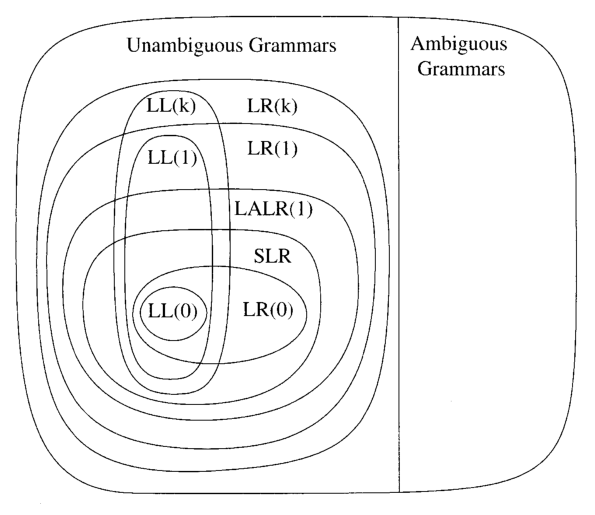
\includegraphics[width=0.5\textwidth]{figures/classesofgrammars.png} % trim=4.85cm 15cm 0.85cm 1cm
\caption{A venndiagram showing the similarities between the different subclasses of CFGs. Where LL(*) is marked with a light blue colour. }\citep{NvidiaCUDASeminar} 
\vspace{-15pt}
\end{figure}
\section{Context free grammar in GAMBLE}
\gls{gamble}'s grammar is written in \acrfull{ebnf}, and uses regular expressions to define terminals such as numbers and identifiers.
In this section there will be a short traversal of a branch from the parse tree.\todo{Hvad ? hvad betyder det??? - Søren}
The full \acrshort{cfg} of \gls{gamble} can be found in \myref{app:CFG} alongside the lexing rules.
This section only presents a small selection of the \acrshort{cfg}.
\gls{gamble}s \acrshort{cfg} is used in the compiler for parsing a program into a structure, which can be manipulated and analysed to produce the target code for the specific program.\todo{Er det vigtigt ? Kan vi ikke nøjes med at sige at grammatikken skal bruges til en parser for gamble ? Vi forklarede det jo i sidste afsnit ? - Søren}
The production rules are used to check for any syntactical errors which might occur.

A production rule from the \acrshort{cfg} of \gls{gamble} is the statement rule. 
Looking at \myref{lst:statements} it is seen that a statement can be both an assignment, declaration, functioncall, controlblock or a loop construct. 
Statement productions are the building blocks of any source code written in \gls{gamble}.

\begin{lstlisting}[caption={\acrshort{cfg} Statement},frame=tlrb,label={lst:statements},numbers=none]
statement
    : assignment ';'
    | declaration ';'
    | functioncall ';'
    | controlblock 
    | loop
    ;
\end{lstlisting}

All production rules in the statement each expand to their own production hence they are non-terminals.
Looking at the declaration production on \myref{lst:declaration} observe that it has two production rules, \texttt{datatype '=' expression} and \texttt{complexdatatype ID '=' expression}. 
They both end on the expression production which can be seen on \myref{lst:expression}.

\begin{lstlisting}[caption={\acrshort{cfg} Declaration},frame=tlrb,label={lst:declaration},numbers=none]
declaration
    : datatype ID '=' expression                        #primitiveDecl
    | complexdatatype ID '=' expression                 #complexDecl
    ; ;
\end{lstlisting}\todo{Er denne rigtig i forhold til den nye grammatik der er blevet lavet igennem tiden ? Den opdaterede grammatik skal også sættes ind i appendix - Søren}

Further expanding into the expression production rules, it can be seen that it has five different production rules.
An expression has production rules expanding the expression into a construct containing more expressions.
This is done because an expression can derive to a value, and several values are needed for multiple arithmetic operations.
This construct also causes left-recursion, something often attempted to be avoided in \acrshort{cfg}.
The parse generator \acrshort{antlr} can handle simple left-recursion as seen on \myref{lst:value} and as such it is acceptable in the \acrshort{cfg} for \gls{gamble}.\todo{Måske vi skal have et afsnit inden gamble CFG omkring parse generators eller noget ? :) Det skal bare nævnes et sted - Søren}
It does so internally rewriting it and as such removes the left-recursion.
\begin{lstlisting}[caption={\acrshort{cfg} Expression},frame=tlrb,label={lst:expression},numbers=none]
expression
    : expression ( '*' | '/' | '%' ) expression     #mulExpr
    | expression ( '+' | '-' ) expression           #addExpr
    | '(' expression ')'                            #parenExpr
    | value                                         #valueExpr
    | ID postUnaryOperator                          #postIDExpr
    ;
\end{lstlisting}
  
The value production rule can expand into what is seen on \myref{lst:value}.
In this production both terminals and non-terminals are included.
The terminals are elements that have no further production rules, leading to a ``dead end''.
When a terminal is reached it is encountered the deriviation ends and the terminal becomes a leaf on the parse tree, also seen in \myref{sec:AST}.
\begin{lstlisting}[caption={\acrshort{cfg} Value},frame=tlrb,label={lst:value},numbers=none]
value
    : ID                                     #valID
    | constant                               #valConstant
    | '[' valueList ( ';' valueList )* ']'   #valList
    | functioncall                           #valFuncCall
    | collectionEntrance                     #valCollectionEntrance
    | BOOLVAL                                #valBool
    ;
\end{lstlisting}\todo{Er de rent faktisk terminals ? Er en terminal ikke noget som ikke har en productionrule ? Det har de vel allesammen her ?}
\todo[inline]{burde vi ikke beskrive alternative labels aka hashtags #? MP}



\chapter{Compiler Overview}
A compiler can be separated into three phases; syntax analysis, contextual analysis and code generation.
The syntax analysis phase checks whether or not the source code adheres to the rules for the language, such as statement constructs.
The contextual analysis phase checks whether or not the language is used correctly, such as type checking.
The code generation translates the source code into the target code once the syntax and contextual analysis phases have accepted the source code.
This chapter examines each phase of the compiler and what these entail.
How each phase is constructed for GAMBLE will also be gone over in this chapter. %This may or may not change
\todo{Mere tekst.}

\label{SourceCodeAsTrees}
\todo{Write about Sourcecode as Trees, and why we do that.}
Error handling is a descriptive section of how the compiler handles errors, and how error handling is implemented.
Error handling is referred to as detection and solving of programming errors.
Both errors at compile time and run time will be handled.
\subsection*{Design}\label{subsec:DesignErrorHandling}
The source code given to the \gls{gamble} compiler may contain errors and warnings, these errors are found and uncovered in various stages of the compiler.   
In the syntax analysis, all syntactic errors are found, and the compilation is stopped if errors are found, since it would not be advised to further compile source code, which contains fundamental syntactic errors.
However it should be noted that the entire syntax analysis is completed before stopping the compiler, hence all syntactic errors are collected and reported to the user.\todo{Et andet sted står der at hvis en fejl mødes bliver det abrupted det skal lige rettes så det passer med det her tror jeg :)(det er vist mig der skrev det bliver stoppet, jeg huskede forkert, I R SOWIE) - Søren}
This makes the process of resolving syntactic errors less tedious for the programmer, than if the compiler would stop every time a single error was detected. 
A core element of error handling is scope and type related errors, these are found in the previously explained subphases of the contextual analysis: Scope- and typechecking.
As with the syntactic analysis, the compiler collects all errors before stopping the compilation of the source code. 
The following errors and warnings are reported by the \gls{gamble} compiler:
\begin{description}
	\item[Argument error]\hfill\\ 
	The arguments required in a function call doesn't match the ones used.
	\item[Redeclaration error]\hfill\\ 
	A variable or function with the same name is already declared.
	\item[Type mismatch error]\hfill\\ 
	The type or types used are incompatible with each other and/or the operator. 
	\item[Undeclared error]\hfill\\ 
	Attempted use of an undefined variable or function.
	\item[Unused variable warning]\hfill\\ 
	A warning signalling that a variable or function is declared but never used.
\end{description} 
The errors in the compiler should give useful information about: Where the error is located in the source code and what variable(s) or function(s) was wrongly used.
This includes line numbers which then have to be carried over from the parse tree to the \acrshort{ast}.

\subsection*{Implementation}\label{subsec:ImplementationErrorHandling}
In the \gls{gamble} compiler the error handling is implemented by having a class \texttt{LanguageError} of which each specific error type inherits from.
The \texttt{LanguageError} superclass has information about the type of the error, an enumeration which is either \texttt{Error} or \texttt{Warning}. 
This is so because a program which has warning but no errors, should still compile, however any program with errors should not. 
Compared to printing any error when it was discovered and stopping compilation, this model allows the compiler to go through the entire \acrshort{ast} and discover every error as described above. 
It also unifies how errors are printed and shown to the user.
There is also an integer indicating which line the error is contained on.
This enhances the error reporting process, making it easier for users to debug. 
As an example the class for \texttt{UnDeclaredError} is shown in \myref{lst:undeclarederrorclass}.
Firstly there are variables which contain information needed to report the error to the programmer. 
Then there is a constructor which simply assigns all values given to it to the new object's fields.
Lastly there is the \texttt{toString} method which is overridden from the implementation in the \texttt{LanguageError} class. 
An example of an \texttt{UnDeclaredError} is: \texttt{Error[line   42]-> Undeclared variable towel in scope Local}, if the variable's ID was \texttt{towel}. %Sneaky H2G2 reference 

\begin{lstlisting}[caption=The UnDeclaredError class in the \gls{gamble} compiler,numbers=none,frame=tlrb,label={lst:undeclarederrorclass}]
public class UnDeclaredError extends LanguageError {
    private Variable unDeclaredVariable;
    private Scope scope;

    public UnDeclaredError(Variable unDeclaredVariable, Scope scope, int lineNum) {
        this.unDeclaredVariable = unDeclaredVariable;
        this.scope = scope;
        this.lineNum = lineNum;
        this.errorType = ErrorType.ERROR;
    }

    @Override
    public String toString() {
        String type = unDeclaredVariable.isFunction() ? "function " : "variable ";
        return super.toString() + String.format("Undeclared %6$s %1$s%4$s%3$s in scope %2$s%5$s%3$s",
                ANSI_RED, ANSI_BLUE, ANSI_RESET,
                unDeclaredVariable, scope, type);
    }
}
\end{lstlisting}

This error is found in the \texttt{CheckIfUndeclared} method in the \texttt{SymbolTableFillVisitor} shown in \myref{lst:CheckIfUndeclared}.
The method is called whenever a variable or function is invoked.
If the variable or function invoked is not declared, an error is added to a global list of errors. 
\begin{lstlisting}[caption=The CheckIfUndeclared method in the SymbolTableFillVisitor class in the \gls{gamble} compiler,numbers=none,frame=tlrb,label={lst:CheckIfUndeclared}]
public Void CheckIfUndeclared(Variable variable, StatementNode node) {
    Symbol tmpSymbol = symbolTable.currentScope().resolve(variable.getId());
    if (tmpSymbol != null) {
        /* Sets appropriate information to the 'variable' variable */
    } else {
        errors.add(new UnDeclaredError(variable, symbolTable.currentScope(), node.getLineNumber()));
        symbolTable.currentScope().define(variable);
    }

    return null;
}
\end{lstlisting}\todo{Stemmer det overens med den nye struktur der blev lavet hvor der kaldes en error class i main ?? - Søren}



\chapter{Syntax Analysis}\label{sec:syntaxAnalysis}
Syntax analysis is the first phase in compiling a language.
In this phase it is checked whether the input adheres to the rules of the language.
These rules are defined in a languages' \acrshort{cfg}.
The \acrshort{cfg} of \gls{gamble} is further described in \myref{sec:cfg} .
This analysis can be split up into to further sub phases, lexical analysis and parsing, these are described in this chapter.
%Design
\section{Design}
\subsection{Scanner}
The first stage of syntax analysis is the scanner, also called the lexer which handles the lexical analysis.
The primary function of a scanner is to transform a sequence of characters into a sequence of tokens.
The scanner makes sure that the source code adheres to the grammar rules provided by the CFG.
An example of this, would be that you could use the notation .1 or 0.1 for a decimal number, both being turned into valid tokens by the scanner.
The scanner provided by ANTLR groups related tokens into token types such as INT, ID and FLOAT.
In ANTLR a token contains at least two pieces of information, the token type and the matched text for the token.

Some examples of our lexical rules for \gls{gamble} can be seen on \myref{lst:token}.
The definition of an integer number on line 3 states that an integer is either a zero or an optional negative sign followed by a single digit from one to nine followed by zero or more numbers from zero to nine.
It is necessary to clearly define tokens for the lexer to read in order to read source code correctly. \citep{Crafting_book}

\begin{lstlisting}[caption=Example of our lexer rules for ANTLR4,frame=tlrb,label={lst:token}]
// Integers
INT: 'int' | 'int16' | 'int32' | 'int64' ; // Integers
INTNUM: '0' | SIGN? [1-9][0-9]* ;

// Matrices and vectors
MATRIX: 'matrix' ;
ROWVECTOR: 'rowvector' | 'rvec' ;
COLVECTOR: 'colvector' | 'cvec' ;  

// Whitespace and comments
WS: [ \t ]+ -> skip;
NL: [ \r \n | \n ] -> skip;

COMMENT
    :   '/*' .*? '*/' -> skip
    ;

LINE_COMMENT
    :   '//' ~[\r\n]* -> skip
    ;
\end{lstlisting}
\subsection*{Parser}\label{subsec:parser}
The parser is based on the \acrfull{cfg} of \gls{gamble} written in \acrfull{ebnf}, whose alphabet consists of tokens produced by the scannar.
The parser reads tokens and groups them into phrases according to the \acrshort{cfg}.
The parser verifies that the syntax is correct and upholds to the \acrshort{cfg}, and if a syntax error is found it provides a corresponding error message. \citep{Crafting_book}
By using a parser generator like \acrshort{antlr} or SableCC, handling of syntactic errors and repairs can be done automatically.
A parser can also be written manually but doing so can result in syntactic errors that is hard to locate or solve.
Writing a parser by hand can also take a lot of time, and it can be difficult to go back and change or add new productions to the syntax, which is something the project group will want to do due to the iterative development.
There are many parser generators which can be used like: SableCC, JavaCC, JFlex and many others, but we have chosen to use \acrshort{antlr}.
\acrshort{antlr} has been chosen due to their special use of the ALL(*) grammar, which poses many opportunities for the grammar, and also makes the \acrshort{cfg} easier to write.
\acrshort{antlr} generates a parser which produces a parse tree that contains information about how the parser have grouped the tokens into more abstract language definitions, such as expressions and statements.

There are different kind of parsers, most common are bottom-up and top-down parsers.
\acrshort{antlr} makes a top-down parser, more specific a recursive descent parser.
A recursive descent parser is a subtype of top-down parser build from a set of mutually recursive procedures where each such procedure implements one of the productions of the grammar.
The structure of the resulting program closely mirrors the grammar it recognizes. \citep{Recursive_programming}
Recursive-descent parsers are a collection of recursive methods, one per rule of the \acrshort{cfg}.
Such a method for an assignment rule may look as shown in \myref{lst:rdpmethod}, where the rule is \texttt{assignment : ID = expr ;}.
So the method expects an ID to be the first token from the tokenstream, then an assignment operator followed by an expression and a semicolon.
Here the expression is a rule itself, and is therefore called on the expected expression.
An error should be returned if anything is not what was expected.
\begin{lstlisting}[caption=Example a recursive descent parser method,frame=tlrb,label={lst:rdpmethod}]
// assign : ID ``='' expr ``;'' ;
void assign() { // method generated from rule assign
match(ID); // compare ID to current input symbol then consume
match('=');
expr(); // match an expression by calling expr()
match(';');
}
\end{lstlisting}

%The second stage of the parser is the actual parser.
%The parser is fed a stream of tokens to recognise a sentence structure and in turn outputs the structure to a parse tree.
%The parse tree records how the parser recognises the structure of the input and its components.
%The parse tree that \acrshort{antlr} provides contains information about how the parser have grouped the tokens into more abstract languange definitions such as expressions and statements.
%Where previous versions of \acrshort{antlr} have also implemented the AST, it is not contained in \acrshort{antlr} V4 instead the parse tree provided by \acrshort{antlr} have been used to generate an AST this is discussed in \myref{sec:AST}.
%This tree is a trimmed version of the parse tree, where the less informative data have been removed, this makes it easier to read, and thus easier to use throughout development of the rest of the compiler.

%2nd stage is the actual parser, feeds of tokens to recognize sentence structure
%Parse tree records how the parser recognized structure of input and its component phrases
%Trees provide an easy to walk data structure that will be helpful for the rest of the compiler
%2.2 Implementing Parser - Recursive descent
%Recursive-descent parsers are really just a collection of recursive methods, one per rule.
%Such a rule may look similar to this
%// assign : ID ``='' expr ``;'' ;
%void assign() { // method generated from rule assign
%match(ID); // compare ID to current input symbol then consume
%match('=');
%expr(); // match an expression by calling expr()
%match(';');
%}
%Descent refers to the fact we start from the root and go down to the leaves(tokens)
%Reursive descent is just one form of top-down parsers.					NOTE topdown/bottom up parsing
%The call graph traaced out by invoking methods, mirrors the interior parse tree nodes
%To Build a parse tree manually one would insert ``add new subroot note' operations at the start of each rule, and a ``add new leaf node'' operation to match()
%The assign method checks if all necessary tokens are present and in the right order. When the parser enters assign it doesnt have to choose between more than one alternative. An alternative is one of the choices on the right side of a rule def. A parsing method for such rule would be a switch which looks for what token is present.
% This is called a parising decision or prediction by examining next token
%This is where lookahead comes into play , the lookahead token is the next input token, this can be any token the parser "sniffs" before consuming
%This is one of the places where \acrshort{antlr} is an especially handy tool to use, because \acrshort{antlr} allows for more lookahead than other parser generators.
%Most parsers use a lookahead of one which LL(1) or LR(1), \acrshort{antlr} tones the lookahead up and down depending on what token stream it is trying to decode, as such the \acrshort{antlr} has a lookahead of LL(*)
%\acrshort{antlr} Solves simple ambiguity simply by using the first mentioned rule.
%AST only useful, Parse all artifacts(space, brackets and so on)


\subsection*{Abstract Syntax Tree}
\todo{to be written}

%Implementation
\section{Implementation}\label{sec:ANTLR}
The syntax analysis is implemented through the tool \acrfull{antlr}, this tool provides some advantages over other available tools.
\acrshort{antlr} is based upon a parser technique called LL(*).
LL(*) uses an algorithm to have a varying lookahead when needed.
The LL(*) parsers, which is a parser that upholds an LL(*) grammar, does not allow a bigger class of \acrshort{cfg}s than other parsers like LL(k), but can change the number of tokens needed as lookahead dynamically. 
In the most recent version of \acrshort{antlr} as time of this publication, \acrshort{antlr}4, the underlying algorithm have been extended to a parser technique called Adaptive LL(*) (ALL(*)).
An important feature of ALL(*) is it moves grammar analysis to parse time and thereby lets the algorithm accept any non-left-recursive productions.
On top of that \acrshort{antlr} allows simple left recursions by rewriting them before parse time.

The \acrshort{antlr} approach accepts a broader class of grammars than most other parsing methods, one way this is done is to rule out ambiguity by using a rule of precedence.
If a grammar is ambiguous the ALL(*) approach will take the first available rule in the \acrshort{cfg} and apply it.
This allows for more opportunities in the \acrshort{cfg} and while most grammars could be rewritten to be unambiguous without applying the precedence rule.
The idea with the ALL(*) algorithm is that the grammar is analysed at parse-time, and requires no static analysis of the grammar. 
This means that the undecidability of static LL(*) grammar analysis is avoided and instead it is possible to make correct parsers for any non-left-recursive \acrshort{cfg}.
This allows \acrshort{antlr} access to input sequences while reading through the grammar, meaning not all possible inputs must be considered.
Due to this dynamic analysis \acrshort{antlr}4 is able to handle some ambiguous constructs and reduce-reduce conflicts.
As mentioned this allows \acrshort{antlr} to take care of left-recursion if such is present in the grammar by rewriting it, as such would be the case in \myref{lst:amb}.

\begin{lstlisting}[caption=An ambiguous rule for expr, which ANTLR handles by applying the first rule of the production if possible,frame=tlrb,label={lst:amb}]
expr : expr '*' expr 	#MulExpression // match expressions with * operator
     | expr '+' expr 	#AddExpression// match expressions with + operator
     | INT 		// matches simple integer
     ;
\end{lstlisting}
\myref{lst:amb} implements \acrshort{antlr}s way of representing operator precedence by simply obeying the first alternative in the rule set, as such the multiplication operator (``*'') will have the higher precedence.
The ALL(*) algorithm also means that one can completely disregard lookahead and it will still be able to parse, although one should keep in mind that having more lookahead than necessary will slow down the process of parsing.
The scanner provided by \acrshort{antlr} groups related tokens into token types such as INT, ID and FLOAT.
In \acrshort{antlr} a token contains at least two pieces of information, the token type and the matched text for the token.
\acrshort{antlr} also implements rule element labels in its \acrfull{cfg} which means one can apply label rules to a construct in a grammar, this allows for conditional steps in the grammar based on the source code being parsed.
The labels on \myref{lst:amb} are \texttt{\#MulExpression} and \texttt{\#AddExpression}.
Furthermore \acrshort{antlr} can set up an interface and base implementation of the visitor pattern for the parse tree on a given grammar by running \acrshort{antlr} with the \texttt{--visitor} flag. \citep{ALLSTAR, LLSTAR, antlr4_Book}

\subsubsection*{Traversal of Trees}
In the previous section an \acrshort{ast} which contains information from the source code was presented; to get the information from the trees, a tree traversal is needed.
For this task different approaches can be taken, one way is to implement a design pattern called the visitor pattern.
Alternatively one can implement the composite pattern or choose to implement no pattern at all, but simply create a case analysis for each object.
The use of a design pattern is not a requirement for the creation of a compiler.

Design patterns provide a general reusable solution for a software problem, each pattern providing its own benefits.
Using a pattern is not just copy and pasting other's code, but it simply states how to solve the problem at hand using different software structures.\todo{Copy pasting code? Hænger det sammen med design patterns? - Corlin}
In OOP, patterns are often described from a UML diagrams, showing the class and interface structure, and which methods these classes must implement. 

The two aforementioned patterns are classified under two different branches of patterns.
The composite pattern is a structural pattern where the visitor pattern is a behavioural one.
A structural pattern provides a way of defining the relations between objects, the composite pattern is used to create a hierarchical recursive tree structure of related objects that may be accessed in a standardised manner.
A behavioural pattern is instead used to define how the objects communicate, the visitor pattern is used to separate a set of structured classes from any functionality that should be performed upon them.\citep{GOF}
For the compiler the visitor pattern have been implemented for the traversal of trees as such the pattern is described further in the following section. 

\subsubsection*{Visitor Pattern}\label{subs:visit}
The visitor pattern is not only used to traverse the parse tree provided by ANTLR, but also the \acrshort{ast} created in the compiler.
The visitor pattern is implemented throughout the compiler, to create the \acrshort{ast} from the parse tree and for traversing the \acrshort{ast}.
As such the visitor pattern defines the structure of the compiler, and thus understanding the benefit from using the pattern is important.
The visitor pattern is described by the Gang of Four, authors of ``Design Patterns: Elements of Reusable Object-Oriented Software'' as:
``a design pattern that separates a set of structured data from the functionality that may be performed upon it.''. \citep{GOF}

In the tree walk for the parse tree, the visitor should convert the parse tree into a \acrshort{ast}.
This entails that each different node in the parse tree must be visited to find the information needed to create the \acrshort{ast}.

Through use of the visitor pattern the functionality is separated from the classes they are performed upon. 
Instead the functionality is on a visitor class implementing the visitor interface, which means different visitors can be made, which all do different computations while traversing the tree.\todo{måske tasks i stedet for computations. MP}
Each class in the tree have an \texttt{accept()} method that allows them to call the visitor in question with itself as an argument.
This allows the ability of adding new operations without changing the original data structure, and also without changing other visitors.
This also serves well when using a iterative development method.
Another benefit is that a single visitor object is used to visit all the classes in the tree.
This visitor can therefore maintain a state between calls to individual data objects, which can be used to save information in an outer scope from the different visit calls.
\myref{image:visitor} shows an UML diagram of the visitor pattern.
This diagram is from a C\# representation, and while the idea is the same the exact implementation is not identical to the one used in the compiler for \gls{gamble}.
Take note of the classes ``ConcreteElement'' and ``ConcreteVisitor''.
The ``ConcreteElement'' represents the different kinds of nodes in a given tree.
The ``ConcreteVisitor'' represents the different kind of visitors implemented.
A visitor will make sure that the children of the node is traversed in the correct way, and will at the same time also do other computations, e.g. pretty printing or checking the source code for errors.\todo{Skal vi komme med andre eksempler her ? Såsom, type checking or code generating?}
A visitor must implement a method to visit every single ``ConcreteElement'' which exist in the tree.
As can be seen on \myref{image:visitor} ``ConcreteVisitorA'' and ``ConcreteVisitorB'', both implement a visit method for the ``ConcreteElements'' A and B.
In the next section, the implementation of creating the \acrshort{ast} from the parse tree using the visitor pattern will be presented.

\begin{figure}[!ht]
\centering
 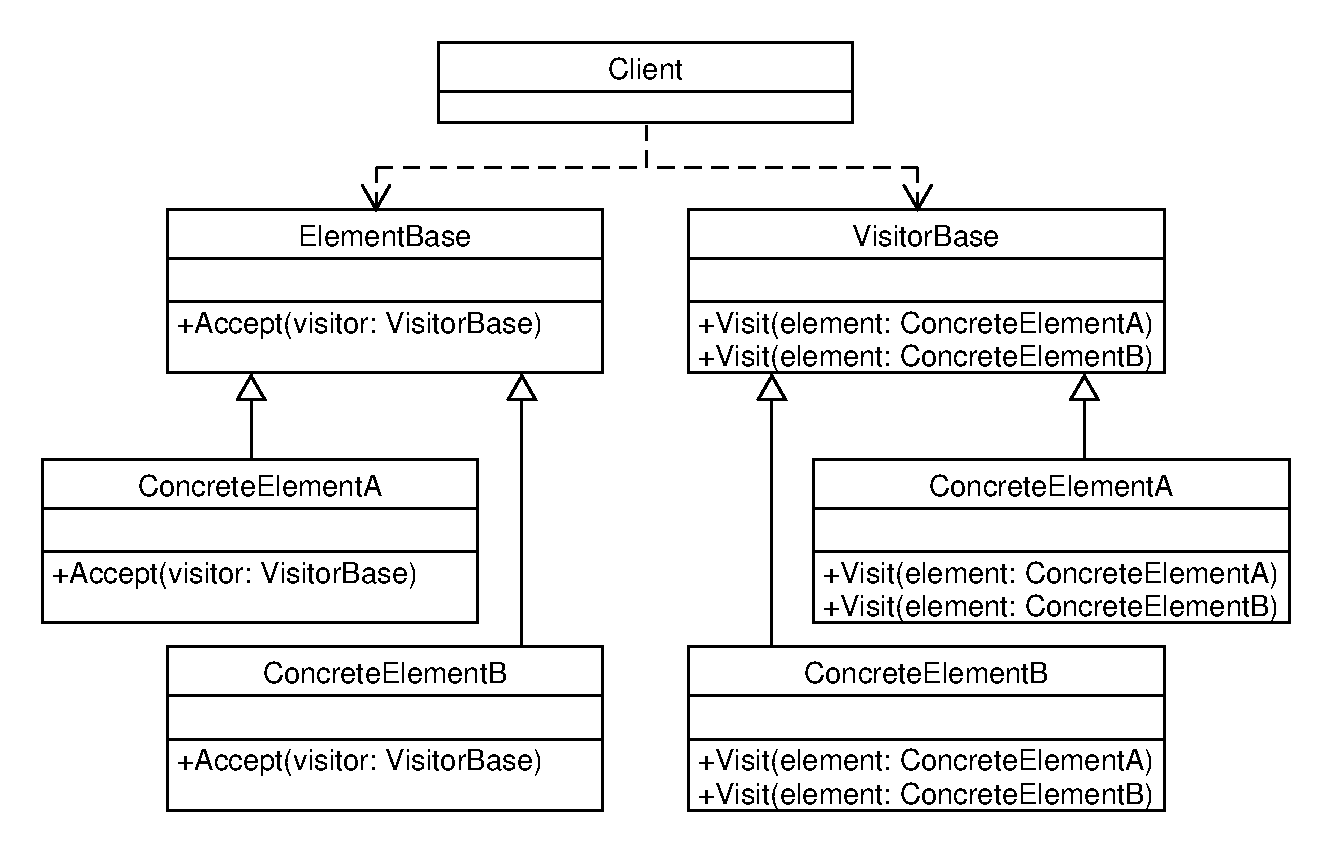
\includegraphics[width=1\textwidth]{figures/ClassDiagrams/VisitorPattern.pdf} % trim=4.85cm 15cm 0.85cm 1cm
\caption{An UML diagram for the implementation of the visitor pattern.}\label{image:visitor}
\vspace{-15pt}
\end{figure}
\todo[inline]{har vi selv lavet figuren? MP - Ja den har jeg lavet :) men der skal nok en kilde på så man kan se hvor vi har det fra, Marc found it. - Søren}

\subsection{Creating the \acrshort{ast}}\label{CreatingAst}

The goal for the \acrshort{ast} is to decrease the information in the tree.
The hidden information is then contained in fields created for the respective classes.\todo{Kan ikke finde ud af om det er lidt for groft at sige hidden information? - Søren}
Rather than having the information as fields one could also choose to have this information as children of the nodes.
This would mean that to find the information one would have to run through the children of the nodes without knowing what children it has.
The method chosen for this compiler has the information kept on the fields of a node rather than as children.
The advantage being that the information is kept together without clustering the tree and increasing the readability of the compiler.
All the nodes of the \acrshort{ast} have been designed with this in mind.
For example on figure \myref{image:ASTDecl} a class structure can be seen, which consists of all the classes needed to express a declaration from the \acrshort{cfg} on the tree.
A declaration could be \texttt{int a = 5;}.

\begin{figure}[!ht]
\centering
 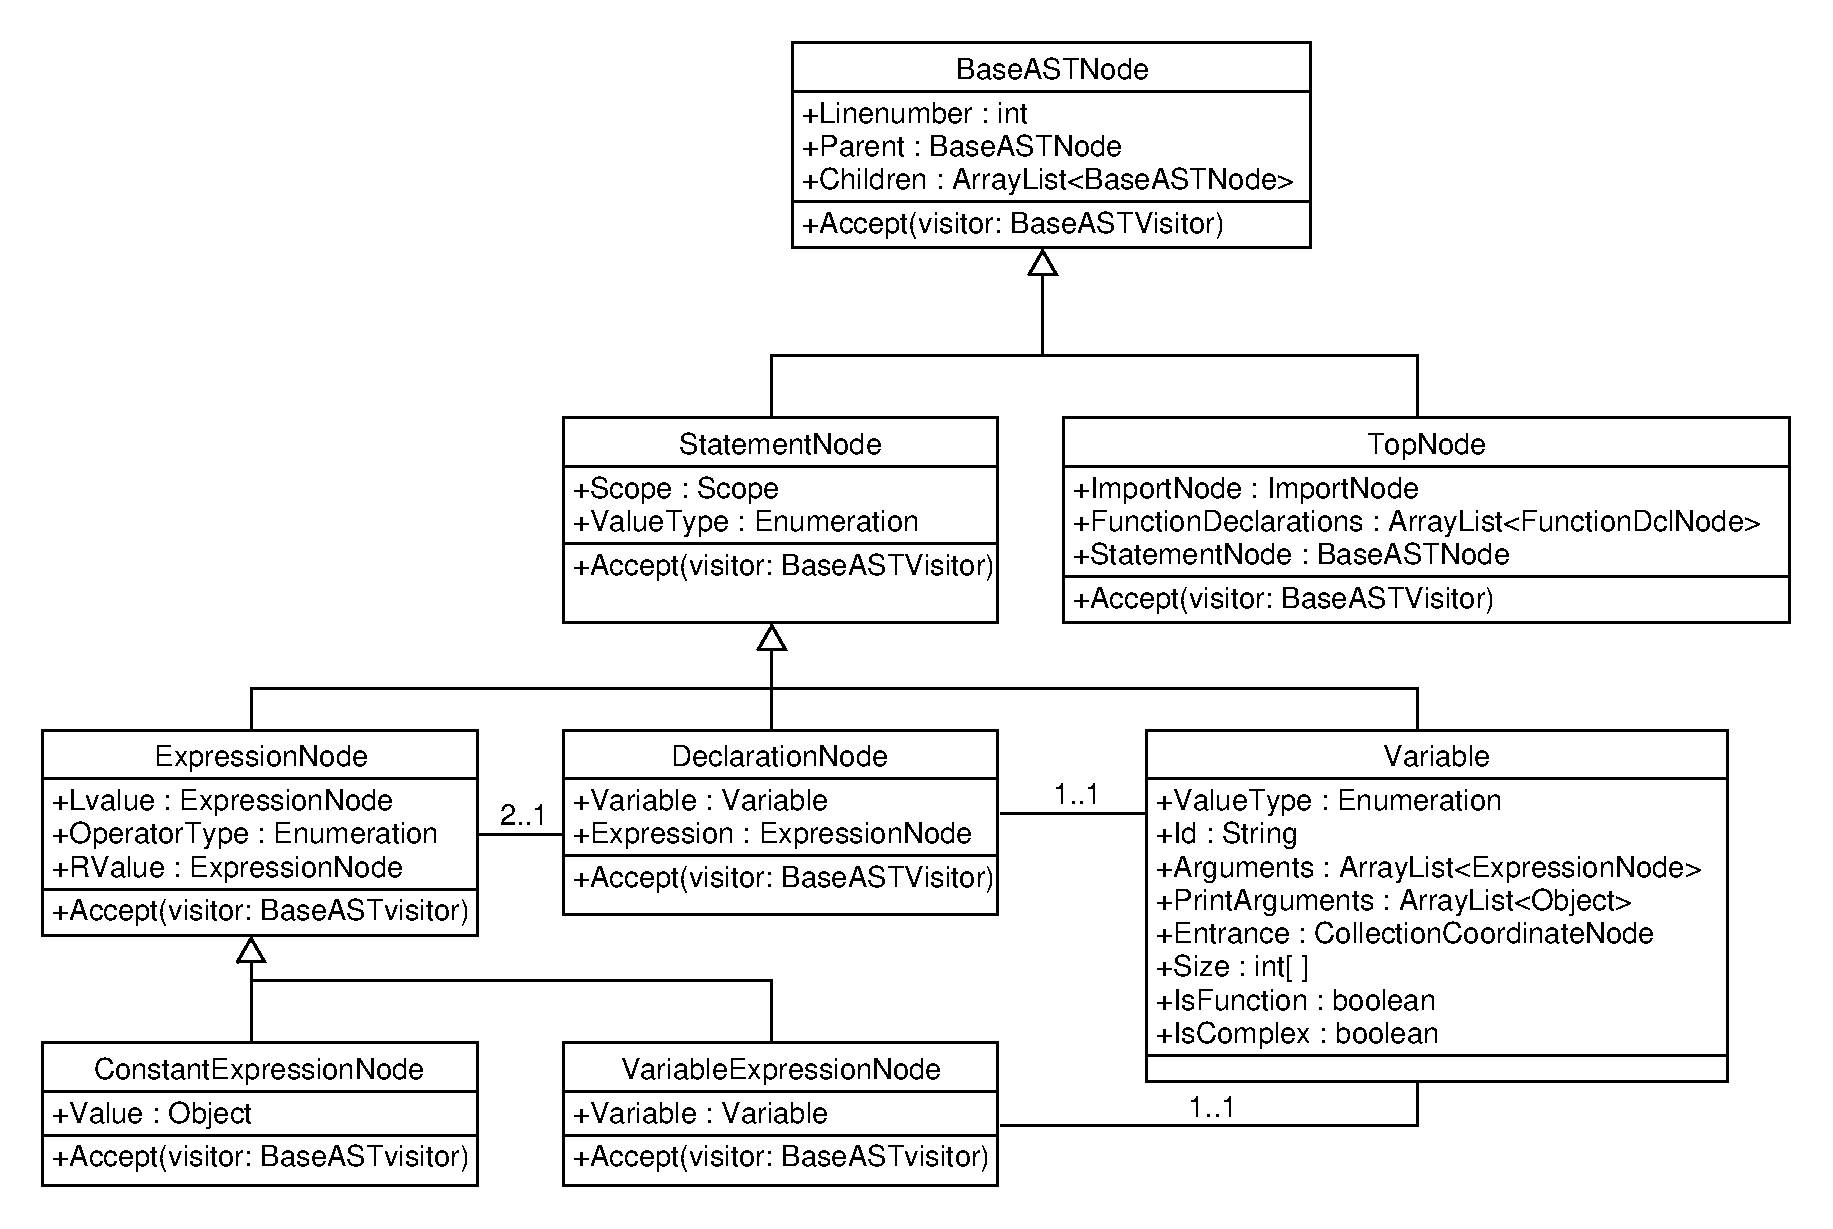
\includegraphics[width=1\textwidth]{figures/ClassDiagrams/ASTDeclarationNodeMoreInfo.pdf} % trim=4.85cm 15cm 0.85cm 1cm
\caption{A UML class diagram of the classes used for a DeclarationNode on the \acrshort{ast}.}\label{image:ASTDecl}
\vspace{-15pt}
\end{figure}

The \texttt{Variable} class contains a lot of different information which is used depending on which class a given instance of \texttt{Variable} is connected to.
If \texttt{Variable} is connected to a \texttt{VariableExpressionNode}, the only fields used on the variable class is ValueType and Id, while the booleans IsFunction and IsComplex are set to false.
In the example \texttt{int a = 5;} the tree structure looks like the AST on \myref{image:AST}.
When the right hand side of an assignment or declaration is a function, an example being \texttt{int a = foo(5);} the fields used on \texttt{Variable} differs from the previous example and instead becomes Id, ValueType, arguments, and the boolean IsFunction is now set to true.
The print argument field is used when a function call to \texttt{print()} is made. 
Entrance, Size and IsComplex are used when dealing with the complex data types, vectors and matrices.
\texttt{TopNode} sets the structure of a \gls{gamble} program as described in \myref{subsec:Struc}.
The full class diagram can be seen in \myref{ASTNodes}.

The classes have made it more intuitive to perform a traversal of the tree based upon the names of the fields on the classes.
E.g. the \texttt{ForLoopNode} has fields named \texttt{Body}, \texttt{Initialize}, \texttt{Update}, and \texttt{Conditional}, these names have meaning instead of just being children on the node which will increases the readability of the compiler.

The syntax analysis phase returns the \acrshort{ast} so it can be used in the next phase, the contextual analysis. 
The design of the phase and the call from main can be seen on \myref{fig:syntaxphase}.\todo{call from main kunne thomas ikke lide. MP - Tror det var fordi han ikke havde set figuren i compiler overview som viser alle kaldene fra main, og dermed var han forvirret over det ? Men ved det self ikke, synes bare ikke det gør noget når man også har set den figur. - Søren}
As can be seen the \texttt{GenerateASTVisitor} makes use of the classes shown in \myref{ASTNodes}.

\begin{figure}[ht]
  \centering
    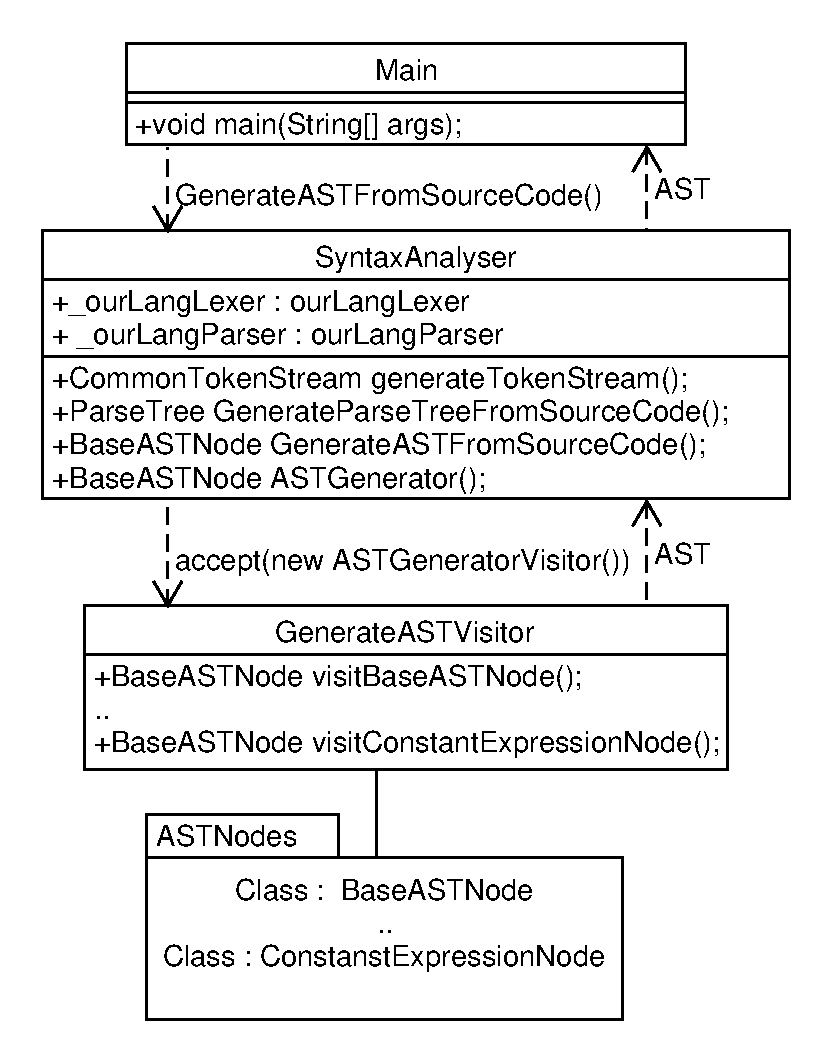
\includegraphics[width=0.48\textwidth]{figures/ClassDiagrams/SyntaxAnalyser.pdf}
  \caption{The function calls and returns in the Syntax Analysis phase.}
  \label{fig:syntaxphase}\todo{Skal vi vise at generateParseTreeFromSourceCode kaldes af ASTFromSourceCode eller noget ? - Søren}
\end{figure}
\subsubsection*{Implementation of Creating the \acrshort{ast}}

The class \texttt{VisitorAST} creates the \acrshort{ast} from the parse tree, it traverses the tree using the visitor pattern and on every node sets a field of a class in the \acrshort{ast}. 
Afterwards the node is placed on the tree as a leaf or a field on the node which made the \texttt{visit()} call.

One of these visit methods can be seen on \myref{lst:VisitorASTCode}.

\begin{lstlisting}[caption=The visit method for WhileLoopNode,frame=tlrb,label={lst:VisitorASTCode}]
public BaseASTNode visitWhileLoop(ourLangParser.WhileLoopContext ctx) {
    WhileLoopNode whileLoopNode = new WhileLoopNode(parentStack.peek());
    whileLoopNode.setCondNode(
    	(ConditionalExpressionNode)visit(ctx.conditionalExpression()));
    parentStack.push(whileLoopNode);
    visitChildren(ctx.whileBlock);
    parentStack.pop();
    whileLoopNode.setLineNumber(ctx.start.getLine());
    return whileLoopNode;
}
\end{lstlisting}
A stack called the parentstack is used to keep track of the caller to \texttt{visit()}, in order to keep track of the parents and the children of the tree.
On lines three and four on \myref{lst:VisitorASTCode} a call to visit the \texttt{conditionalexpression} of the whileloop is made, which returns an instance of the class \texttt{ConditionalExpressionNode}.
Afterwards, to set the body of the \texttt{WhileLoopNode}, all the children of the nodes are visited, but first the \texttt{WhileLoopNode} is pushed to the parentstack.
This makes it possible to check which node is the parent of the children being created during the calls to visit.
\acrshort{antlr} uses the implementation where each node has a number of children, and therefore the \texttt{WhileLoopContext} has its children visited rather than specific fields.
While implementing the Visitor pattern for the \acrshort{ast} an interface was made, which contains a visit method for every single class of the \acrshort{ast}.
A baseclass which implements this interface which implements a visit method for all the nodes of the \acrshort{ast} such that the correct fields of the nodes are visited in the intended order.
This means that any visitor class only has to override the visit methods which are of interest for the specific visitor and the ones not overridden will use the baseclass' implementation which simply visits its fields.
An UML diagram for the implementations of the visitor pattern in the compiler and can be seen on \myref{image:Visitors}.
The figure shows how every visitor class inherits from the \texttt{BaseASTVisitor} class.\todo{Overvejer lidt om denne figur skal væk da det jo er design og egentlig bare viser det som figuren i design viser? - Søren}
Now that the Syntax analysis phase is done it is time for the \acrshort{ast} to be send to the contextual analysis phase which the next chapter will cover.

\begin{figure}[!ht]
\centering
 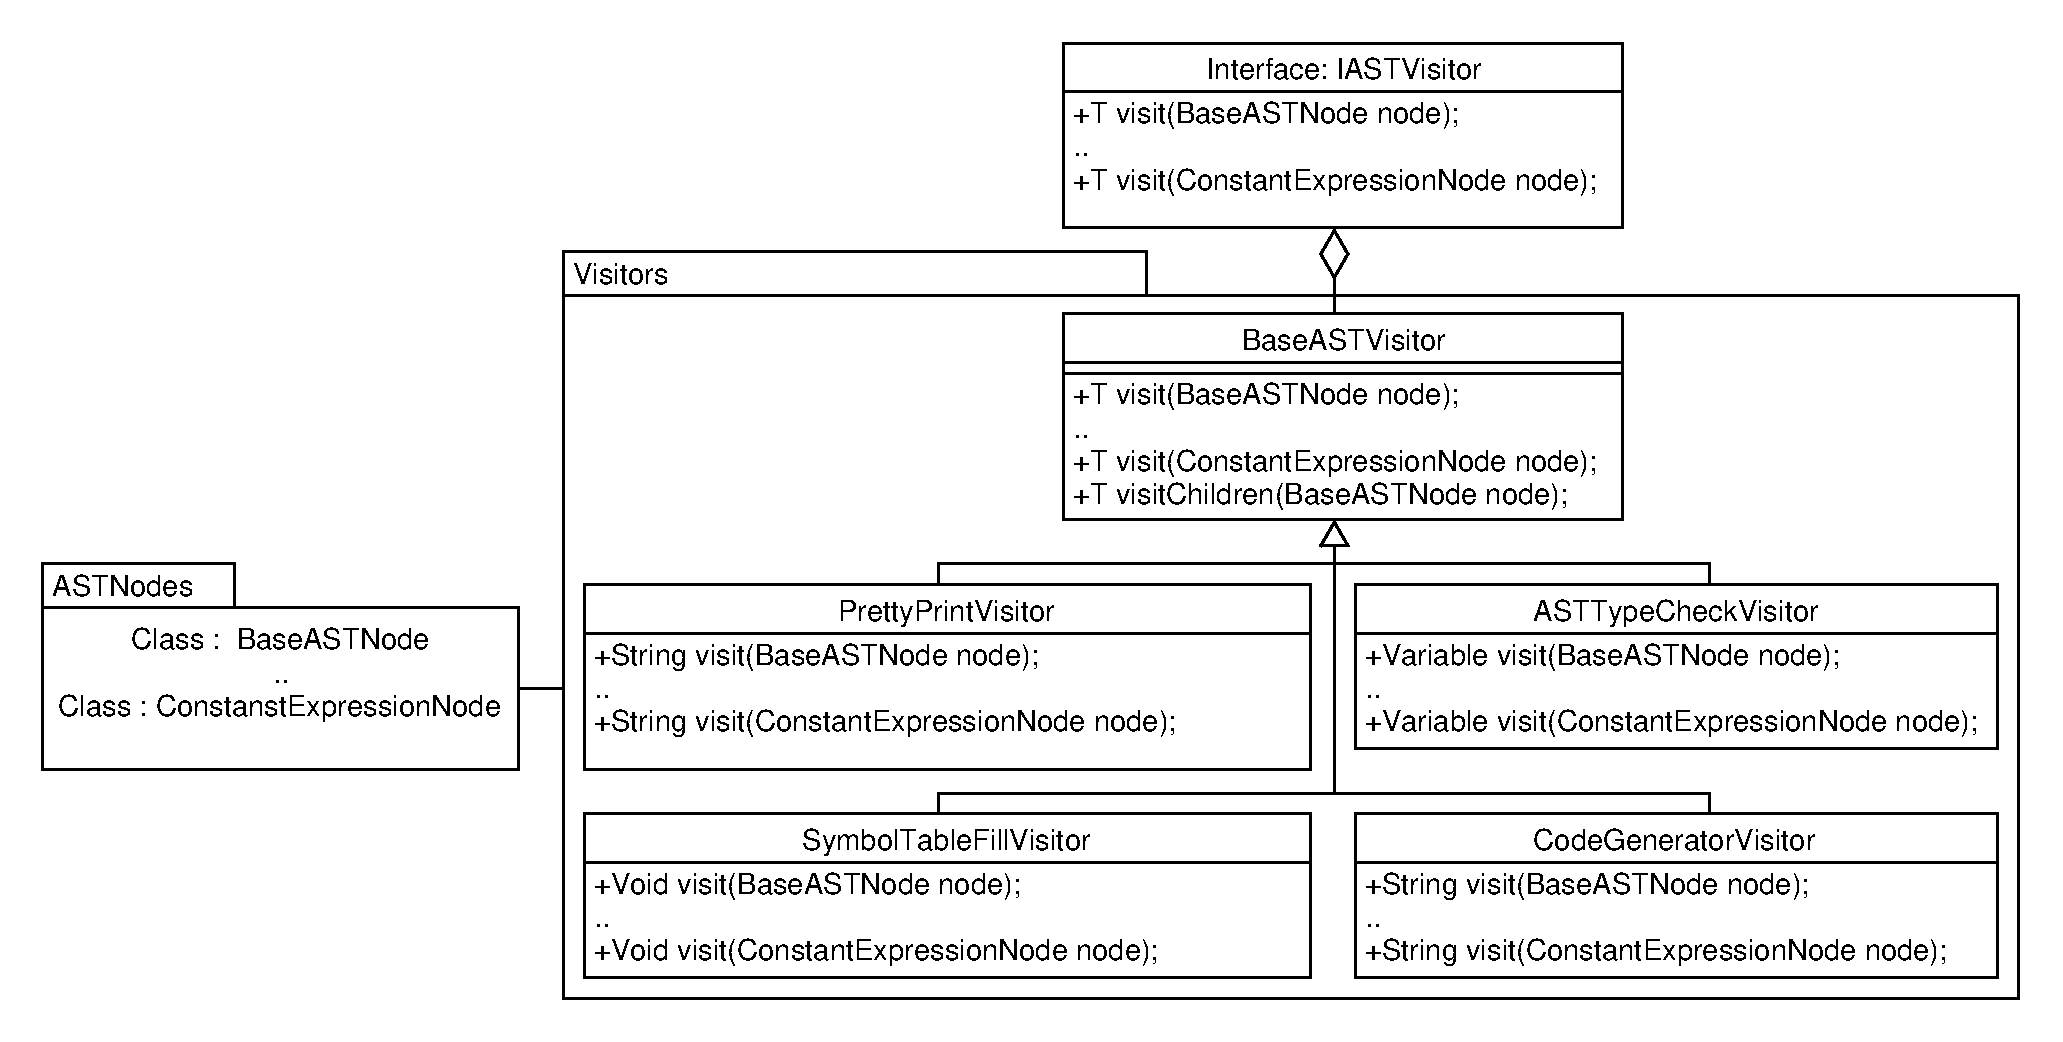
\includegraphics[width=1\textwidth]{figures/ClassDiagrams/Visitors.pdf} % trim=4.85cm 15cm 0.85cm 1cm
\caption{An UML diagram of the visitor patterns implementation in the compiler for traversing the \acrshort{ast}.}\label{image:Visitors}
\vspace{-15pt}
\end{figure} 

%Subphases
\chapter{Contextual Analysis}
\section{Contextual Analysis}
\info[inline]{meta for this, phases are done in their own subsection files}
\section{Symbol Table}
In a compiler it is useful to store information about the identifiers, variables and functions in a data structure. 
This information can be useful for scope checking and type checking.

There are two common ways of implementing a Symbol Table; either you have one table which contains every identifier or you have a Symbol table for each scope. 
If constrained by memory, having a single symbol table can be beneficial, however having multiple symbol tables can simplify the code at a memory cost. 

In \gls{gamble} there exists scopes, and for each of these scopes there is a corresponding symbol table. 
Scopes inherit from each other so a scope can enclose another. 
The outermost scope, the global scope, is where functions are declared; every scope is either directly enclosed by this scope or recursively.
This means that every function can be called from anywhere within the source code - including within its' own function declarations; allowing for recursive functions. 
  

\info[inline]{Flyttes til implementationsafsnit $\downarrow$ }
In \gls{gamble} the class \texttt{SymbolTable} represents the symbol table.
The core constituent of this class is the ArrayList of the Scope class, called allScopes, meaning that every scope is stored in this ArrayList.
Every scope contains Map of Symbols and strings as keys, and information about the scope such what scope it is enclosed by. 
The key represents the name of the symbol, and must be unique to the scope and not found in an enclosing scope, as this could cause an ambiguity to arise. 
A symbol is either a variable or a function, in the class Symbol its data type, name and scope is stored. 


\section{Scope Checking}
As a part of the contextual analysis the compiler must ensure that every reference is valid in their given scope.
The validity of such reference is specific to the rules of the language, this section describes how the compiler upholds the rules listed in \myref{subsec:Scope}.
\subsection*{Design}
In \myref{subsec:Scope} the scope of identifiers, variables and functions, are defined for \gls{gamble}.
A variable is in scope from its declaration until the end of the block it is declared in.
An inner scope inherits the identifiers declared in the outer scopes. 

In the contextual analysis part of the compiler it is important to verify that each variable and function used are in scope, and it should produce a useful error message.
The error message should indicate which identifier is not in scope, and on what line this identifier is used wrongly.

To check this all references to identifiers must be checked to see if they match an identifier in the symbol table of the current scope, and recursively the scope which encloses it. 
Furthermore it is important that any usage of an identifier only exists after its declaration.
In the compiler for this project, the symbol table is filled while the compiler is also performing the scope checking.
This is because it reduces the amount of traversals through the tree, and scope checking and filling the symbol table is also similair in concept, e.g. a declaration creates an entry in the symbol table, while expressions simply make lookups in this table.

The scope checker produces two errors: redeclaration errors and undeclared errors.
A redeclaration error is produced when an attempt to declare a variable while it is already declarared in scope is made.
An undeclared error is produced when an attempt to use a variable which is not declared in the current scope or any enclosing scopes is made. 
Examples are shown in \myref{lst:scopeErrors}.

\begin{lstlisting}[caption=Examples of scope errors in \gls{gamble}, numbers=none,frame=tlrb,label={lst:scopeErrors}]
/* [...] */
int a = 1;
float a = 2.2;   /* Redeclaration error */
int a = 2;       /* Redeclaration error */ 

b = 2;           /* Undeclared error */   
int b = 0;
b = foo();       /* Redeclaration error and undeclared error */ 
/* [...] */
\end{lstlisting}

\subsection*{Implementation}
In the \gls{gamble} compiler, the class \texttt{SymbolTable} represents a collection of scopes.
The core constituent of this class is the ArrayList of the \texttt{Scope} class, called \texttt{allScopes}, meaning that every scope is stored in this ArrayList.
Every scope contains a hashed map with \texttt{Symbol}s as values and strings as keys.
Furthermore all scopes contain information about the particular scope such as enclosing scope and a unique id. 
The key in the hashed maps represents the name of the symbol, and must be unique to the scope and not found in an enclosing scope, as this could cause an ambiguity to arise.
This ambiguity is not allowed in \gls{gamble} and therefore generates a redeclaration error.
To determine wether or not a declaration is a redeclaration, the compiler looks up the name of the variable in the \texttt{symbolMap} of the current scope.
If no entry is found, the search continues in the \texttt{symbolMap} of the enclosing scope and outwards.
The same lookup process is executed when a variable is used e.g in a expression or assignment.
Hereby all enclosing scopes are checked for the declaration of the variable; making redeclaration of variables in scope, and usage of undeclared variables impossible in \gls{gamble}.
A symbol is an encapsulation of a variable and relevant peripheral data.
The peripheral data consists of a boolean, used for checking is a declared variable is used, and an integer with the line number if the declaration of the variable.
The boolean describing if a declared variable is used, is set to true, if the previously described lookup process for a variable in use, finds a declared variable from the unique id (the name if the variable).
This boolean also makes it possible for the \gls{gamble} compiler to find unused variables and then prompt the user with a relevant warning.

In order for all of the above to be implemented an instance of the \texttt{SymbolTable} class is passed via the constructor, to a visitor which traverses the \acrfull{ast}.
This visitor, the \texttt{SymbolTableFillVisitor} then fill the referenced \texttt{symbolTable} with scopes and their symbols.
Every time the visitor meets the start of a new scope e.g. the block of statements within a loop construct.
A new instance of the \texttt{Scope} class is pushed to the \texttt{scopeStack}, hereby making it possible to fill the relevant scope when the block of statements is visited.
At the end of a scope the top element on the \texttt{scopeStack} is popped off, and as a consequence of this the top of the \texttt{scopeStack} is back to the enclosing scope.

\section{Type Checking}
\subsection*{Design}
The second important part of the contextual analysis phase for the compiler is the type checking, which enforces the type system of \gls{gamble}.
As \gls{gamble} is statically typed it is necessary to check if all references to identifiers and constant values fit into the context they exist in. 
Since implicit conversion between floating point and integer types is not a part of \gls{gamble} an error must be issued everywhere they are used wrongly. 
It is however possible to implicitly convert between integer and floating point types internally e.g. from int16 to int64, as long as the destination variable is of a larger bit-width.
This is also the case for complex datatypes, matrices and vectors, e.g. from \texttt{matrix<float>} to \texttt{matrix<float64>}. 

The symbol table is used as a reference for which type the variable is, and therefore the type checking happens after the symbol table has been filled, hence after scope checking is completed. 
Type checking is done in many parts of the code, one or more times for each line is common. 
For every operator it must be checked if its types match and if it results in an assignment if that also matches.
Every function call must match the formal parameters of the function. 

The errors produced by the type checker are: Argument errors and type mismatch errors.
An argument error indicates that the number of arguments in the function declaration does not match the number of arguments provided in the function call.
A type mismatch error is caused by a value or identifier not being compatible (type safe) with the function parameters, operator used etc.
Examples are shown in \myref{lst:typeErrors}.

\begin{lstlisting}[caption=Examples of type errors in \gls{gamble},numbers=none,frame=tlrb,label={lst:typeErrors}]
/* [...] */
int a = 1 + 2;      /* Valid */
float b = 2.2 + 1;  /* Type mismatch error */
float c = 2;        /* Type mismatch error */

a = 2.2;            /* Type mismatch error */
b = foo(1);         /* Argument error (Takes more or fewer arguments) */ 
/* [...] */
\end{lstlisting}

\subsection*{Implementation}
The type checker is called right after the symbol table has been filled by the \texttt{SymbolTableFillVisitor}.
Since \gls{gamble} is static typed, the type checker is implemented under the contextual analysis phase of the compiler, in contrast to a dynamically typed language, such as Python or R, which is checked at runtime. \todo{er dette nødvendigt. MP}
\gls{gamble} validates the size of matrices and vectors match for certain operations as addition and multiplication E.g., as well as if they are out of bounds. 
This is to make it easier for the programmers using \gls{gamble} at a cost of speed. 
To implement type checking in the \gls{gamble} compiler a visitor is used during the contextual analysis.
The class \texttt{ASTTypeCheckVisitor} visit every relevant node in the \acrshort{ast} to check for type errors.
The class collects a list of every type error it finds, these errors is then presented to the user, when a compilation fails.
Errors and error handling are further described in \myref{subsec:DesignErrorHandling}.
The class \texttt{ASTTypeCheckVisitor} overrides the visitor calls from the \texttt{baseASTVisitor} class.
The visitor does this in multiple places in the \acrshort{ast} and the visitor uses a class \texttt{TypeChecker}, which through method calls on the variables in the nodes.
\texttt{TypeChecker} contains a method, \texttt{CombineValueTypes} which takes two values and checks if they are type compatible.
\texttt{ASTTypeCheckVisitor} visits nodes which contains either one or more variables meaning that there can be errors which should be found. 
An example of this is seen in \myref{lst:typecheck1} where the method \texttt{VisitExpressionNode}
 is shown.
The method visits an \texttt{ExpressionNode} and calls \texttt{CombineValueTypes} with the nodes left and right values if there are any available else it send \texttt{null} as the input value.
The method visits an \texttt{ExpressionNode} and uses the the \texttt{TypeChecker}s \texttt{CombineValueTypes} method, the method checks the types of the children of the \texttt{ExpressionNode} and if they fits the operator then it returns the type of the expression. 
The method returns a variable of the type returned \texttt{ValueType} and string which is printed if the visit finds type errors.

\begin{lstlisting}[caption=The VisitExprressionNode method in the ASTTypeChecker class,numbers=none,frame=tlrb,label={lst:typecheck1}]
public Variable VisitExpressionNode(ExpressionNode node) {
    ValueType valueType = TypeChecker.CombineValueTypes(
            node.getLValue() != null ? visit(node.getLValue()) : null,
            node.getRValue() != null ? visit(node.getRValue()) : null,
            errors,
            node.getLineNumber()
    );
    node.setValueType(valueType);

    return new Variable(valueType, "Expr:<" + node.toString() + ">");
}
\end{lstlisting}

After the type checker have checked every expression in the source code, the compiler scans for unused variables and thereafter prints all these as warnings. 

\section{Error Handling}
Error handling is a descriptive section of how the compiler handles errors, and how error handling is implemented.
Error handling is referred to as detection and solving of programming errors.
Both errors at compile time and run time will be handled.
\subsection*{Design}\label{subsec:DesignErrorHandling}
The source code given to the \gls{gamble} compiler may contain errors and warnings, these errors are found and uncovered in various stages of the compiler.   
In the syntax analysis, all syntactic errors are found, and the compilation is stopped if errors are found, since it would not be advised to further compile source code, which contains fundamental syntactic errors.
However it should be noted that the entire syntax analysis is completed before stopping the compiler, hence all syntactic errors are collected and reported to the user.\todo{Et andet sted står der at hvis en fejl mødes bliver det abrupted det skal lige rettes så det passer med det her tror jeg :)(det er vist mig der skrev det bliver stoppet, jeg huskede forkert, I R SOWIE) - Søren}
This makes the process of resolving syntactic errors less tedious for the programmer, than if the compiler would stop every time a single error was detected. 
A core element of error handling is scope and type related errors, these are found in the previously explained subphases of the contextual analysis: Scope- and typechecking.
As with the syntactic analysis, the compiler collects all errors before stopping the compilation of the source code. 
The following errors and warnings are reported by the \gls{gamble} compiler:
\begin{description}
	\item[Argument error]\hfill\\ 
	The arguments required in a function call doesn't match the ones used.
	\item[Redeclaration error]\hfill\\ 
	A variable or function with the same name is already declared.
	\item[Type mismatch error]\hfill\\ 
	The type or types used are incompatible with each other and/or the operator. 
	\item[Undeclared error]\hfill\\ 
	Attempted use of an undefined variable or function.
	\item[Unused variable warning]\hfill\\ 
	A warning signalling that a variable or function is declared but never used.
\end{description} 
The errors in the compiler should give useful information about: Where the error is located in the source code and what variable(s) or function(s) was wrongly used.
This includes line numbers which then have to be carried over from the parse tree to the \acrshort{ast}.

\subsection*{Implementation}\label{subsec:ImplementationErrorHandling}
In the \gls{gamble} compiler the error handling is implemented by having a class \texttt{LanguageError} of which each specific error type inherits from.
The \texttt{LanguageError} superclass has information about the type of the error, an enumeration which is either \texttt{Error} or \texttt{Warning}. 
This is so because a program which has warning but no errors, should still compile, however any program with errors should not. 
Compared to printing any error when it was discovered and stopping compilation, this model allows the compiler to go through the entire \acrshort{ast} and discover every error as described above. 
It also unifies how errors are printed and shown to the user.
There is also an integer indicating which line the error is contained on.
This enhances the error reporting process, making it easier for users to debug. 
As an example the class for \texttt{UnDeclaredError} is shown in \myref{lst:undeclarederrorclass}.
Firstly there are variables which contain information needed to report the error to the programmer. 
Then there is a constructor which simply assigns all values given to it to the new object's fields.
Lastly there is the \texttt{toString} method which is overridden from the implementation in the \texttt{LanguageError} class. 
An example of an \texttt{UnDeclaredError} is: \texttt{Error[line   42]-> Undeclared variable towel in scope Local}, if the variable's ID was \texttt{towel}. %Sneaky H2G2 reference 

\begin{lstlisting}[caption=The UnDeclaredError class in the \gls{gamble} compiler,numbers=none,frame=tlrb,label={lst:undeclarederrorclass}]
public class UnDeclaredError extends LanguageError {
    private Variable unDeclaredVariable;
    private Scope scope;

    public UnDeclaredError(Variable unDeclaredVariable, Scope scope, int lineNum) {
        this.unDeclaredVariable = unDeclaredVariable;
        this.scope = scope;
        this.lineNum = lineNum;
        this.errorType = ErrorType.ERROR;
    }

    @Override
    public String toString() {
        String type = unDeclaredVariable.isFunction() ? "function " : "variable ";
        return super.toString() + String.format("Undeclared %6$s %1$s%4$s%3$s in scope %2$s%5$s%3$s",
                ANSI_RED, ANSI_BLUE, ANSI_RESET,
                unDeclaredVariable, scope, type);
    }
}
\end{lstlisting}

This error is found in the \texttt{CheckIfUndeclared} method in the \texttt{SymbolTableFillVisitor} shown in \myref{lst:CheckIfUndeclared}.
The method is called whenever a variable or function is invoked.
If the variable or function invoked is not declared, an error is added to a global list of errors. 
\begin{lstlisting}[caption=The CheckIfUndeclared method in the SymbolTableFillVisitor class in the \gls{gamble} compiler,numbers=none,frame=tlrb,label={lst:CheckIfUndeclared}]
public Void CheckIfUndeclared(Variable variable, StatementNode node) {
    Symbol tmpSymbol = symbolTable.currentScope().resolve(variable.getId());
    if (tmpSymbol != null) {
        /* Sets appropriate information to the 'variable' variable */
    } else {
        errors.add(new UnDeclaredError(variable, symbolTable.currentScope(), node.getLineNumber()));
        symbolTable.currentScope().define(variable);
    }

    return null;
}
\end{lstlisting}\todo{Stemmer det overens med den nye struktur der blev lavet hvor der kaldes en error class i main ?? - Søren}


%Phase3
\chapter{Code Generation}
Code generation is the phase in which the object code is generated, the process and considerations this entails are covered in this chapter.
Object code is the output of the compiler.
Once the source code has passed through syntax analysis and contextual analysis without errors it has been validated and the compiler can proceed with generating the object code.
In the case of this compiler the object code is OpenCL C, as a result one or more compilers beyond this one are required to eventually end up with machine code that can be executed.\todo{more compilers? - e.g. vi bruger vores egen og gcc - Marc}
The object code is OpenCL C this means that tasks such as instruction selection and scheduling as well as register allocation will be handled by the compiler which will compile the OpenCL C code rather than \gls{gamble}.\todo{Håndterer compileren scheduling ????? - Søren - Instruction scheduling var en af de nævnte ting fra SPO kurset som man på lavniveau håndtere ja - Marc .. instruction scheduling er jo hvilken rækkefølge en given sekvens af instruktioner udføres i, ikke hvilken process har adgang til CPUen på et givent tidspunkt. -- Troels}
Furthermore in the code generation phase optimisation of the object code also takes place, for \gls{gamble} this means to create object code which is quickly executed and utilises the \acrshort{gpu} for calculation that benefit from its use.\todo{er det ok at bruge optimisation her, vi code gen'er jo bare, det er jo ikke rigtig en optimering. ? :) - Søren - Men området er referet til som optimisation, det er også derfor der efter står hvad betydningen af optimisation er for gamble - Marc }
A state diagram showing the sub-phases of the code generation can be seen in \myref{fig:flowCodegen}.

\vspace{10pt}
\begin{figure}[h]
    \centering
    \begin{tikzpicture}[node distance = 3cm, auto]
        %\node (invi1) [invi, draw=none] {};
        %\node (ast) [lille, below=-0.35cm of invi1] {Abstract Syntax Tree};
        %\node (symboltable) [lille, minimum width=6.75cm, minimum height=2.4cm, right=2cm of invi1, fill=blue!10, label={[xshift=0cm, yshift=-1cm]Symbol Table}] {};
        %\node (scope) [lille, right=1.1cm of ast] {Scopechecker};
        %\node (type) [lille, right=0.7cm of scope] {Typechecker};
        %\node (dast) [lille, right=1.1cm of type] {Decorated Abstact Syntax Tree};

        %\node (error) [cloud, below=1cm of symboltable] {Error report};

        %\draw [arrow] (ast) -- (scope);
        %\draw [arrow] (scope) -- (type);
        %\draw [arrow] (type) -- (dast);
        %\draw [arrow,dashed] (scope) -- (error);
        %\draw [arrow,dashed] (type) -- (error);
        %\draw [arrow,dashed] (symboltable) -- (error);

        \node (dast) [lille, align=left] {Contextual \\Analysis Phase};
        \node (cgv) [lille, right=0.7cm of dast, align=left] {Code Generation \\Visitor};
        \node (copy) [lille, right=0.7cm of cgv] {Output \gls{opencl} C code};
        \node (error) [invi, draw=none, minimum width=2cm, right=1cm of copy, label={[xshift=40pt, yshift=-17pt]Finished Compilation}] {};

        \draw[black,fill=black, above=1cm of parser] (10.9,0) circle (1ex);
        \draw[black, above=1cm of parser] (10.9,0) circle (1.3ex); 

        \draw [arrow] (dast) -- (cgv);
        \draw [arrow] (cgv) -- (copy);
        \draw [arrow] (copy) -- (error);
    \end{tikzpicture}
    \caption{State diagram showing the modules of the code generation. } 
    \label{fig:flowCodegen}
\end{figure}
\vspace{-20pt}

\subsection*{GPU Usage}\label{GPUCode}
Since \gls{gamble} distances its programmers from directly controlling which computations are performed on the \acrshort{gpu}, determing what code to perform on the \acrshort{gpu} becomes a problem for the compiler to solve.\todo{task, lyder bedre eller hvad? MP. - tasks synes jeg ikke rigtigt passer en når det er hvilke kodesegmenter, måske operations hvis det skal ændres? - Marc}
To make this decision the compiler must know what kind of code performs faster on a \acrshort{gpu} than a \acrshort{cpu}.

From \myref{sec:comparch} it is clear that for it to make sense to move any computation to the \acrshort{gpu} it must be of significant size to make up for the overhead of moving data, and be executable in parallel.
If a computation is reliant on the outcome of other computations, the Fibonacci function as an example, moving it to the \acrshort{gpu} would be a significant decrease in performance compared to a \acrshort{cpu}.

Any code written in a recursive format will not be run on the \acrshort{gpu}. 
Furthermore due to the overhead in data transfer, only computations requiring a significant amount of operations to be performed should be executed on the \acrshort{gpu} as \myref{image:benchmark} shows.
Therefore statements which only contain simple data types, i.e. integers, floats and booleans, are performed on the \acrshort{cpu}.
An example could be \texttt{value = value1 + value2}, where all types are integers.
%Therefore statements not containing complex data types, i.e. statements with no vector or matrix arithmetics, are also performed on the \acrshort{gpu}.

However statements that do include matrix or vector arithmetics will be performed on the \acrshort{gpu}.
An example could be matrix multiplication.
Now it is entirely possible to make a matrix multiplication of a $2\times2$ matrix, which would be so small that the overhead of data transfer is more expensive than simply computing on the \acrshort{cpu}. \todo{Det er jo ikke kune data overførslen som koster tid? Der er også JIT af kernel i nogle cases (se alle). -- Troels}
However to simplify the code generation it has been chosen that all matrix or vector calculations, are to be done on the \acrshort{gpu}.
This is not always the best choice, as \myref{sec:comparch} clearly shows, but it requires less analysis of the code given, furthermore as mentioned in \myref{sec:phil} \gls{gamble} uses the \acrshort{gpu} to gain computational power for performing already developed algorithms on data sets big enough to see an improvement in execution time.
Also even if smaller matrices are being computed, the increase in runtime is significantly less than the decrease for just a single bigger matrix operation, as can be seen on \myref{fig:test_results}.
\todo[inline]{Måske nævne vi hellere vil flytte små matricer på gpu, end at beholde store på cpuen? MP - God ide, den tid det tager at flytte en lille matrix til GPU er heller ikke så stor som det man spare på at flytte store matricer til gpu'en. - Søren - Som ovenstående? - Marc}



\info[inline]{next chapters are : Test of language, Conclusion, and Perspektivaaation(top kek)}
  
\chapter{Test of Language} % (fold)
\label{cha:test_of_language}
In order to evaluate upon the capabilities of \gls{gamble} a test is run. 
As performance of mathematical operations is in focus, the project group has chosen to only test the language by comparing the execution time of using the \acrshort{gpu} with the execution time of using the \acrshort{cpu} sequentially.

Previously handwritten C code for the \acrshort{cpu} has been compared to handwritten CUDA C code running on the \acrshort{gpu}, see \myref{sub:gpubenchmark}.
The results of this test can within reason be expected to have a similar output, meaning that at low data sizes the \acrshort{cpu} is faster than the \acrshort{gpu}, however as the size of the data gets bigger the \acrshort{gpu} is faster.
The reason for the \acrshort{gpu} being slow for low data sizes is that memory needs to be allocated on the \acrshort{gpu}, the input data must be copied to the \acrshort{gpu}, the calculation must be done, and then the data can be copied back to main memory. 
Once in main memory the data can be further processed e.g. written to a file. 
This means that a relatively high amount of time will not be used for calculations, but for moving data back and forth from main memory to the memory of the \acrshort{gpu}.
The hypothesis from the previous test in \myref{sub:gpubenchmark} was that a more computation heavy test would be faster on the \acrshort{gpu} on smaller sizes, so the intersection of the 2 lines would be for a smaller value on the x-axis. 
The reason for this hypothesis is that because of the large overhead cost the more computations done with the data once it is available in the \acrshort{gpu} will increase the speed of execution compared to the sequential implementation on a \acrshort{cpu}.

It is to be noted that neither the code for the \acrshort{cpu} nor the \acrshort{gpu} is optimised by anything other than the gcc-compiler, as explained in \myref{ssub:makefile}. 
This means that the code could be made faster at execution time, for example by loop-unrolling, multi-core use with threading etc. for the \acrshort{cpu}, and by varying the size of the work group, offline kernel compilation, advanced memory use i.e. local and private memory, for the \acrshort{gpu}.  

\section{The Test} % (fold)
\label{sec:the_test}
The performed test is a simple matrix multiplication with non square matrices.
For the \acrshort{gpu} the built-in matrix operation in \gls{gamble} for matrix multiplication is used. 
The syntax for this operation is: \texttt{matrixA * matrixB}. 
This construction is compiled to a kernel which is invoked for each index in the result matrix, the kernels each calculate just one index of the resulting matrix, and has an inner loop of the size of the columns of the first matrix, which is equal to the rows of the second matrix.
To replicate this for the \acrshort{cpu}, a construct with three nested for-loops is used, where the inner most loop is similar to the one found in the dedicated kernel, and the two outer loops are used to execute the inner loop for each index in the resulting matrix.
Hence the \acrshort{cpu} and \acrshort{gpu} targeted code does the same number of calculations.
 
As an example, with square matrices, of size $n$ as input the amount of calculations is $2*n^3 = O(n^3)$ operations. 
And there are $3*n^2 = O(n^2)$ numbers in the matrices which will be operated on, $2/3$ will be read from and $1/3$ will be written to.

When testing execution time, especially on \acrshort{cpu} intensive programs, there is a lot of different variables in the equation. 
The scheduler of the operating system and IO-requests can slow down the execution while caching and cache hits can speed up the computations because of faster memory access. 
These factors will in this test be regarded as the benefits and disadvantages that follows when using the \acrshort{cpu} for compute intensive tasks.
Because of this, trend lines will be used to visualise the data points along with the raw plots. 

\subsection{Test Environment} % (fold)
\label{sub:test_environment}
The test for the \acrshort{cpu} is written in C, and the \acrshort{gpu} test is of course written in \gls{gamble}.
As previously mentioned the \acrshort{gpu} focused side of the test, will be using the built-in matrix multiplication of \gls{gamble}, and the \acrshort{cpu} side, the three nested for-loops.
The sizes of the matrices are changed using a script which starts the programs where the matrices are given different dimensions and the time result is appended to a file.

The test will be executed on a machine running Ubuntu 14.04.2 LTS, with an Intel Core i5-4670K overclocked to 4.5 GHz as the \acrshort{cpu} and an AMD R9 280x with 3GB of GDDR5 ram and a clock of 1070 MHz as the \acrshort{gpu}.
As the main memory 8 GB of DDR3 ram is available for the programs.
For running the test on a range of different matrix sizes, a bash script will be used to alter the dimensions through the previously mentioned text files, which will then be loaded by the programs as matrices.
Sourcecode for both programs along with the script used for testing, can be found in \todo{tilføj til apen(dicks)}.

\subsection{Results} % (fold)
\label{sub:results}
After running the test and visualising the execution time for the different matrix sizes, it is clear that the \acrshort{gpu} performs better than the \acrshort{cpu}.
In the graph below (\myref{fig:test_results}), we see that the line representing the \acrshort{gpu} is located well below the line representing the \acrshort{cpu}.   
\begin{figure}[h!]
    \centering
    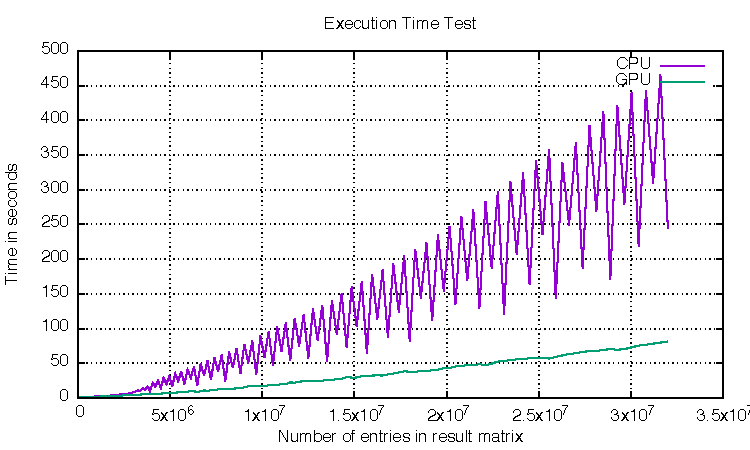
\includegraphics{figures/tests/graph.pdf}
    \caption{Execution time of matrix multiplication, with sequential \acrshort{cpu} and heterogeneous \acrshort{gpu} approach}\label{fig:test_results}
\end{figure} 
It should however be noted that in the beginning of the graph (the leftmost side), the two lines are very close to each other since time measurements are less precise at such low numbers, and the overhead of initialising and allocating memory for the matrices can well exceed the raw computation time of the multiplication.     
Furthermore the line representing the \acrshort{cpu} is very jagged, which indicates that the aforementioned caching are influencing the execution time.
Be that as is may, the \acrshort{gpu} is always faster in execution time at performing matrix multiplication compared to the \acrshort{cpu} especially when the number of entries in the result matrix exceeds $5*10^6$.
If doing other operations like adding or multiplying a scalar, the results might have been different and looked more like the results from \myref{sub:gpubenchmark}

% subsection results (end)
% section the_test (end)

% chapter test_of_language (end) 
\chapter{Conclusion} % (fold)
\label{cha:conclusion}
During the project different aspects of the process of creating a language and a compiler or interpreter have been presented.
Different ways of handling these aspects have been discussed as well as the implementation of these.
The language \gls{gamble} was designed to make it easier for programmers and mathematicians alike to perform matrix and vector computations that used the power of the \acrshort{gpu} without the programmer needing to specify so in the source code.
It was chosen that a compiler would be the best fit for translating the \gls{gamble} language.
Using the operators, defined in \myref{subsec:operators}, along with matrices or vectors \gls{gamble} will compile to \gls{opencl} C code, which runs the computations on the \acrshort{gpu}.
As a result of running computations on the \acrshort{gpu} an increase in runtime efficiency can be obtained.
An increase in runtime efficiency will only exist if the computations are of a significant size. \myref{cha:test_of_language} shows what data size is required for \gls{gamble} to provide an increase in runtime efficiency by using the \acrshort{gpu} rather than the sequential execution on the \acrshort{cpu}.

\myref{cha:language_criteria} mentions the criteria that the project group set for \gls{gamble} and what became its compiler.
The runtime efficiency test for \gls{gamble} concludes that \gls{gamble} can run faster than the sequential C code, at least for the operations \gls{gamble} performs on the \acrshort{gpu}.
The way \gls{gamble} is designed, this happens seamlessly to the programmer which was also a criterion for the language.
When the \acrshort{gpu} usage happens seamlessly it increases both the read- and writability of the language, because of the removal of all the boiler-plate code needed for executing on the \acrshort{gpu}.
Another criterion was to implement an error reporting system which would give descriptive error messages to ease the debugging of programs compiled by the compiler.
This is done by making a number of standard error classes for scope and type checking, and creating instances of these when encountering a corresponding error in the \acrshort{ast} in the contextual analysis phase, and continuing the scope and type checking until completion.
When the phase is complete the compiler will have a list of all the errors encountered and can print these in the console with the type of error and also the line number where the error occurs.
Another result of the contextual analysis phase is that it makes sure that programs written in \gls{gamble} and compiled by the \gls{gamble} compiler will run reliably according to the scope and type rules of \gls{gamble}.
Further testing of the compiler has been performed which tests whether the specifics of \gls{gamble}'s type and scope checking work as intended, making sure that the correct error messages are shown when they need to be as seen in \myref{cha:test_of_language_features}.
This test further tests for the correctness of the compiled code.
These tests test if code made in \gls{gamble} acts as expected and give the expected result.
The results of these tests indicate that the operators of \gls{gamble}, the scope checker and the type checker are working as intended 

For creating the parser for the compiler, the parser generator \acrshort{antlr}4 was used.
\acrshort{antlr}4 made a parser from the \acrshort{cfg} specified by the project group.
This parser generates a parse tree which is translated into an \acrshort{ast} by the compiler.
The \acrshort{ast} removes redundant information from the parse tree thus simplifying its traversal.
The \acrshort{ast} allowed for easier access to the nodes than the parse tree, while grouping information and using less nodes for information compared to the parse tree.
Scope and type checking are essential parts of the compiler and identifies errors in the source code before runtime.

The project showed that there are many aspects in creating a language and a compiler.
The use of the \acrshort{gpu} is worthwhile when the size of the computations become sufficiently large, and creators of new languages or compilers should think of including ways of using this resource for such purposes.
Furthermore it became evident that attempting a general solution for all \acrshort{gpu} platforms is not the best approach, it would be better to spend the proper amount of time developing for each individual platform, if that time is available.


Based on the test of the language using the compiler and the fact that it upholds all the criteria stated by the project group, it is concluded that the solution is satisfactory.
The usage of an iterative development method has proven to be a good choice for the project group as it allowed the group to change and add features as the project progressed and more knowledge was acquired.
However the knowledge of \gls{opencl}.s limitations was acquired too late, and there was not enough time for the group to switch to \gls{cuda} before the project deadline.
The choice of a modular compiler design would make the switch to \gls{cuda} C or any other target language simpler and easier.
\chapter{Future Works}\label{cha:future_works}
While the language and compiler functionality is complete in the sense of this paper, one can always expand.
In this chapter some of the possible expansions, i.e. new features and optimizations, will be discussed.

\section{Linear Algebra}\label{improve:LIAL}
%More operations
%More algortihms
During development of \gls{gamble} the focus have laid upon linear algebra.
As such incorporating more operations such as finding the inverse matrix, would remove the necessity of the programmers themselves having to develop functions to do so.
Moreover this would make it easier to implement algorithms which makes use of such operations.
Further development could also include some of the most common algorithms e.g. Gaussian elimination.
As a result of how the \acrshort{gpu} is used in the current version of \gls{gamble}, the operations and functions created by the programmer, may very well use the \acrshort{gpu} but not as much, nor as effectively as it could.
Therefore making these improvements to the core language, would not only increase the writability of \gls{gamble}, but also increase the overall performance on run-time.

\section{GPU Usage Criteria}
%A more dynamic use of GPU through analysis
%Use GPU for more than matrix and vector operations
As aforementioned \gls{gamble} performs all operations between matrix and vector on the \acrshort{gpu}.
While this should be sufficient for computations on big sets of data as the language has targeted, this is not the optimal solution.
A possible expansion would be to optimize further to only utilize the \acrshort{gpu} when an increase in performance is to be expected from doing so.
An analysis of the amount of computations required as well as the hardware available, would help towards gaining the best performance possible.
Even further development should also look further than only performing matrix and vector operations on the \acrshort{gpu}.
This was chosen because that all operations currently implemented towards doing matrix and vector operations are parallelizeable.
If implementing new operations and functions one must consider whether these benefit from the use or \acrshort{gpu} or not.
For further development of \gls{gamble} one should also consider using the \acrshort{gpu} for more than matrix and vector operations and hereby developing the language to do \acrshort{gpgpu}. 
Rather than blindly disregarding loops one could have the compiler check whether or not the loop in question could be parallelised, and perhaps perform some of the optimizations mentioned in \myref{optimisation} upon said loop.
 
\section{Kernel Efficiency}
%Kernal optimisation
When creating kernels one must allocate memory within the memory hierarchy established in the OpenCL framework.
In this compiler all memory is allocated in global memory as it significantly simplifies the knowledge of the \acrshort{gpu} hardware and its memory hierarchy required to write kernels.
With a deeper understanding of how the different memory sections communicate, it is possible to increase performance by using the best suited part of the memory hierarchy. \citep{ocl_lecture3}

\section{Platform Specifications}
%Platform performance
While OpenCL is not machine dependant, which machine one is working on does change what version of OpenCL is supported, as well as how different work sizes and data types are handled.
An example would be that while AMD \acrshort{gpu}s have hardware to support both integer and float calculations, NVIDIA \acrshort{gpu}s only uses floats. \citep{CUDAOpenCLOptimisation}
Due to these discrepancies the same program and kernel may perform differently on \acrshort{gpu}s with the same specifications but from different vendors.
As such, different implementations depending on manufacturer and OpenCL support may increase performance depending on the specific hardware.

\section{Scientific Computing}
%From LIAL to Scientific computing
While making it possible to perform linear algebra operations have been the focus of this compiler, this is not the only field of computing that can benefit from the computational powers of the \acrshort{gpu}.
Graph theory, molecular dynamics, computational chemistry and many other fields all include compute intensive simulations and number crunching.
Further developing the language to fit yet another field would significantly increase the use for such a language in the scientific community.
As long as one can ensure that the computations required can in some form be parallelised such that the \acrshort{gpu} can be of use, this is a possible and large addition to the language.
Alternatively one could be content with adding new data types and operations for other fields and implement the field specific methods as libraries.
This would make the language usable by other fields, as the users would be able to implement the needed methods themselves.
%Er ikke helt vild med formulering af line 47 og 49, men synes ikke lige jeg kan formulere det anderledes at the time of writing dis.

\section{Expand \gls{gamble} to be more general purpose}
At this point \gls{gamble} is rather narrowly focused on certain areas like matrix and vector operations, the language could benefit from being expanded to become a more general purpose language.
In the following paragraphs some of the key aspects to expand the language are discussed.

\gls{gamble} does not have general collection types which could benefit many program types.
Examples of such collection types could be \texttt{struct}, \texttt{list} or \texttt{array}.
These additions would allow the programmer to implement abstract data structures such as trees.

A full implementation of strings would also be beneficial for a more general purpose language.
In extension to proper strings a reassessed print method could be rewritten to allow the programmer to format the printing of variables to the like of other languages such as C.

Making \gls{gamble} object oriented with common features like inheritance and polymorphism would allow many programmers to write programs similar to what they are used to.
This would make it easier to write large programs.

Libraries for the language could also be beneficial and increase the expressibility of \gls{gamble}.
An example of a library could be a math library to allow different mathematical constructs and expressions currently not supported by the language.
Such a library could include operations like square root, cosine and sine among others.
A more complex mathematical library could allow more complex operations of the complex data types vectors and matrices.

Another way of expanding the language would be to utilise the similarity between matrices and graphics and therefore implement libraries to perform image processing of graphics.
These libraries could therefore use similar ways of using the \acrshort{gpu} as matrices already do.
\printglossaries
\bibliography{bib/mybib}
\label{bib:mybiblio}

\appendix
\chapter{GPU overhead}
\label{app:gpuoverhead}
To reach an approximation for when a GPU can run a program faster than a CPU  we wrote two equivalent programs.
The first with C as source code and the second as a C source code with CUDA libraries to preform calculations on the GPU.
Both program was run on a desktop computer with an i5 3570k processer and GTX 660 Ti graphics card.

The programs performs different operations on a square matrix of size n, then we ran the program for multiple n's between 100 and 20000.

The operations on the matrix can be seen on \myref{gpuoversource}, the full source code of the two programs can be found on the CD-ROM on \myref{app:cd}.

\begin{lstlisting}[language=C,caption={Operations on the matrix},label=gpuoversource,frame=single]
for (i = 0; i < dim; i++) {
	for (j = 0; j < dim; j++) {
		a[i*dim+j] *= a[i*dim+j];
		a[i*dim+j] -= a[i*dim+j] / 2.0;
		a[i*dim+j] /= dim / 2;
		a[i*dim+j] += a[i] * 2;
	}
}
\end{lstlisting}

 %label app:gpuoverhead
\chapter{CD-ROM}
\label{app:cd}
See attached CD below %label app:cd
\chapter{CFG}\label{app:CFG}
\begin{lstlisting}[caption={\acrshort{cfg} and Lexing rules},frame=tlrb,numbers=none]
//PARSER

topLevel
    : importing* functiondeclaration* statement* EOF
    ;

statement
    : assignment ';'
    | declaration ';'
    | functioncall ';'
    | controlblock
    | loop
    ;

importing
    : IMPORT '<' LIBRARY '>'
    ; 

controlblock
    : IF '(' conditionalExpression ')' block (ELSE IF '(' conditionalExpression ')' block)* (ELSE block)?
    ;

loop
    : WHILE '(' conditionalExpression ')' block
    | FOR '(' (declaration | assignment) ';' conditionalExpression ';' expression ')' block
    ;

block
    : '{' statement* '}'
    ;
                                                                       
conditionalExpression                                                  
    : conditionalExpression '&&' conditionalExpression                 
    | conditionalExpression '||' conditionalExpression                 
    | expression conditionalOperator expression                        
    | conditionalExpression  ( '==' | '!=' ) conditionalExpression     
    | '(' conditionalExpression ')'                                    
    | BOOLVAL                                                          
    ;                                                                  
                                                                       
functiondeclaration
    : functiondatatype ID '(' parameterlist ')' functionbody
    ; 
    
functionbody
    : '{' ( statement )* functionreturn? '}'
    ;

functionreturn
    : 'return' expression ';'
    ;

parameterlist
    : (parameter( ',' parameter )*)?
    | 
    ;

parameter
    : (valueType | complexdatatype ) ID
    ;                                      
                                           
functioncall                               
    : ID '(' argumentlist ')'              
    | PRINT '(' argumentlist ')'           
    | COMPLEXTOFILE '(' argumentlist ')'   
    | FILETOCOMPLEX  '(' argumentlist ')'  
    ;                                      

argumentlist
    : (expression | STRING) ( ',' (expression | STRING) ) *
    | 
    ;

expression                                            
    : expression '^' expression                       
    | expression ( '*' | '/' | '%' | '#' ) expression 
    | expression ( '+' | '-' ) expression             
    | '(' expression ')'                              
    | value                                           
    | ID postUnaryOperator                            
    ;                                                 
                                                      
assignment
    : valassignment
	| collectionassignment
    ;

valassignment                                       
	: ID assignmentOperator ( expression | BOOLVAL )
    | ID postUnaryOperator                          
	;                                               
                                                       
collectionassignment                                   
	: ID '=' expression                                
	| collectionEntrance assignmentOperator expression 
	;                                                  
	
declaration                                           
    : valueType ID '=' expression                     
    | complexdatatype ID '=' expression               
    | complexdatatype '[' entranceCoordinate ']' ID   
    ;                                                 
    
valueType                          
    : INT                          
    | FLOAT                        
    | BOOL                         
    ;                              
                                   
complexdatatype
    : collectiontype '<' valueType '>'
    ;

functiondatatype
    : valueType
    | complexdatatype
    | VOID
    ;

value                                      
    : ID                                   
    | constant                             
    | '[' valueList ( ';' valueList )* ']' 
    | functioncall                         
    | collectionEntrance                   
    | BOOLVAL                              
    ;                                      
                                           
collectionEntrance
    : ID '[' entranceCoordinate ']'
    ;

valueList
    : value ( ',' value)*
    ;

constantList
    : constant ( ',' constant )*
    ;

entranceCoordinate
    : value ( ',' value )?
    ;

collectiontype
    : MATRIX   
    | VECTOR    
    ;

postUnaryOperator 
    : '++' | '--' | '^T' ;

assignmentOperator
    : '=' | '+=' | '-=' | '*=' | '/=' ;

conditionalOperator
    : '==' | '!=' | '<=' | '>=' | '<' | '>' ;

constant
    : INTNUM  
    | FLOATNUM 
    ;

//LEXER  

IMPORT: 'include' | 'import' ;  
  
IF: 'if' ;
ELSE: 'else' ;

WHILE: 'while' ;
FOR: 'for' ;   
PFOR: 'pfor' ;

MATRIX: 'matrix' ;
VECTOR: 'vector' ;

INT: 'int' | 'int16' | 'int32' | 'int64' ;
INTNUM: '0' | SIGN? [1-9][0-9]* ;

FLOAT: 'float' | 'float16' | 'float32' | 'float64' ;  
FLOATNUM: SIGN? ([1-9][0-9]* | '0') '.' ([0-9]* [1-9] | '0') ;

BOOL: 'bool' ;
BOOLVAL: 'true' | 'false' ;

VOID: 'void' ;

STRING: '"' .*? '"' ;

SIGN: '-' ;   

PRINT: 'print' ;
COMPLEXTOFILE: 'matrixToFile' ;
FILETOCOMPLEX: 'fileToMatrix' ;

ID: [a-zA-Z_][a-zA-Z0-9_]* ;    

LIBRARY: [a-zA-Z0-9_\/'.']+;

//Whitespace and comments

WS: [ \t ]+ -> skip;

NL: [ \r \n | \n ] -> skip;

COMMENT
    :   '/*' .*? '*/' -> skip
    ;

LINE_COMMENT
    :   '//' ~[\r\n]* -> skip
    ;
                                                
\end{lstlisting} %label app:CFG
\chapter{Abstract Syntax Tree Class Diagram}\label{ASTNodes}
In this Appendix the full class diagram of the \acrshort{ast} used for the compiler, can be found.
All associations have been colored red, except if they cross over other red lines, then one of them is colored blue so it is easier to follow the associations on the figure found on the following page.
\begin{sidewaysfigure}   
\vspace{-10pt}
\centering
 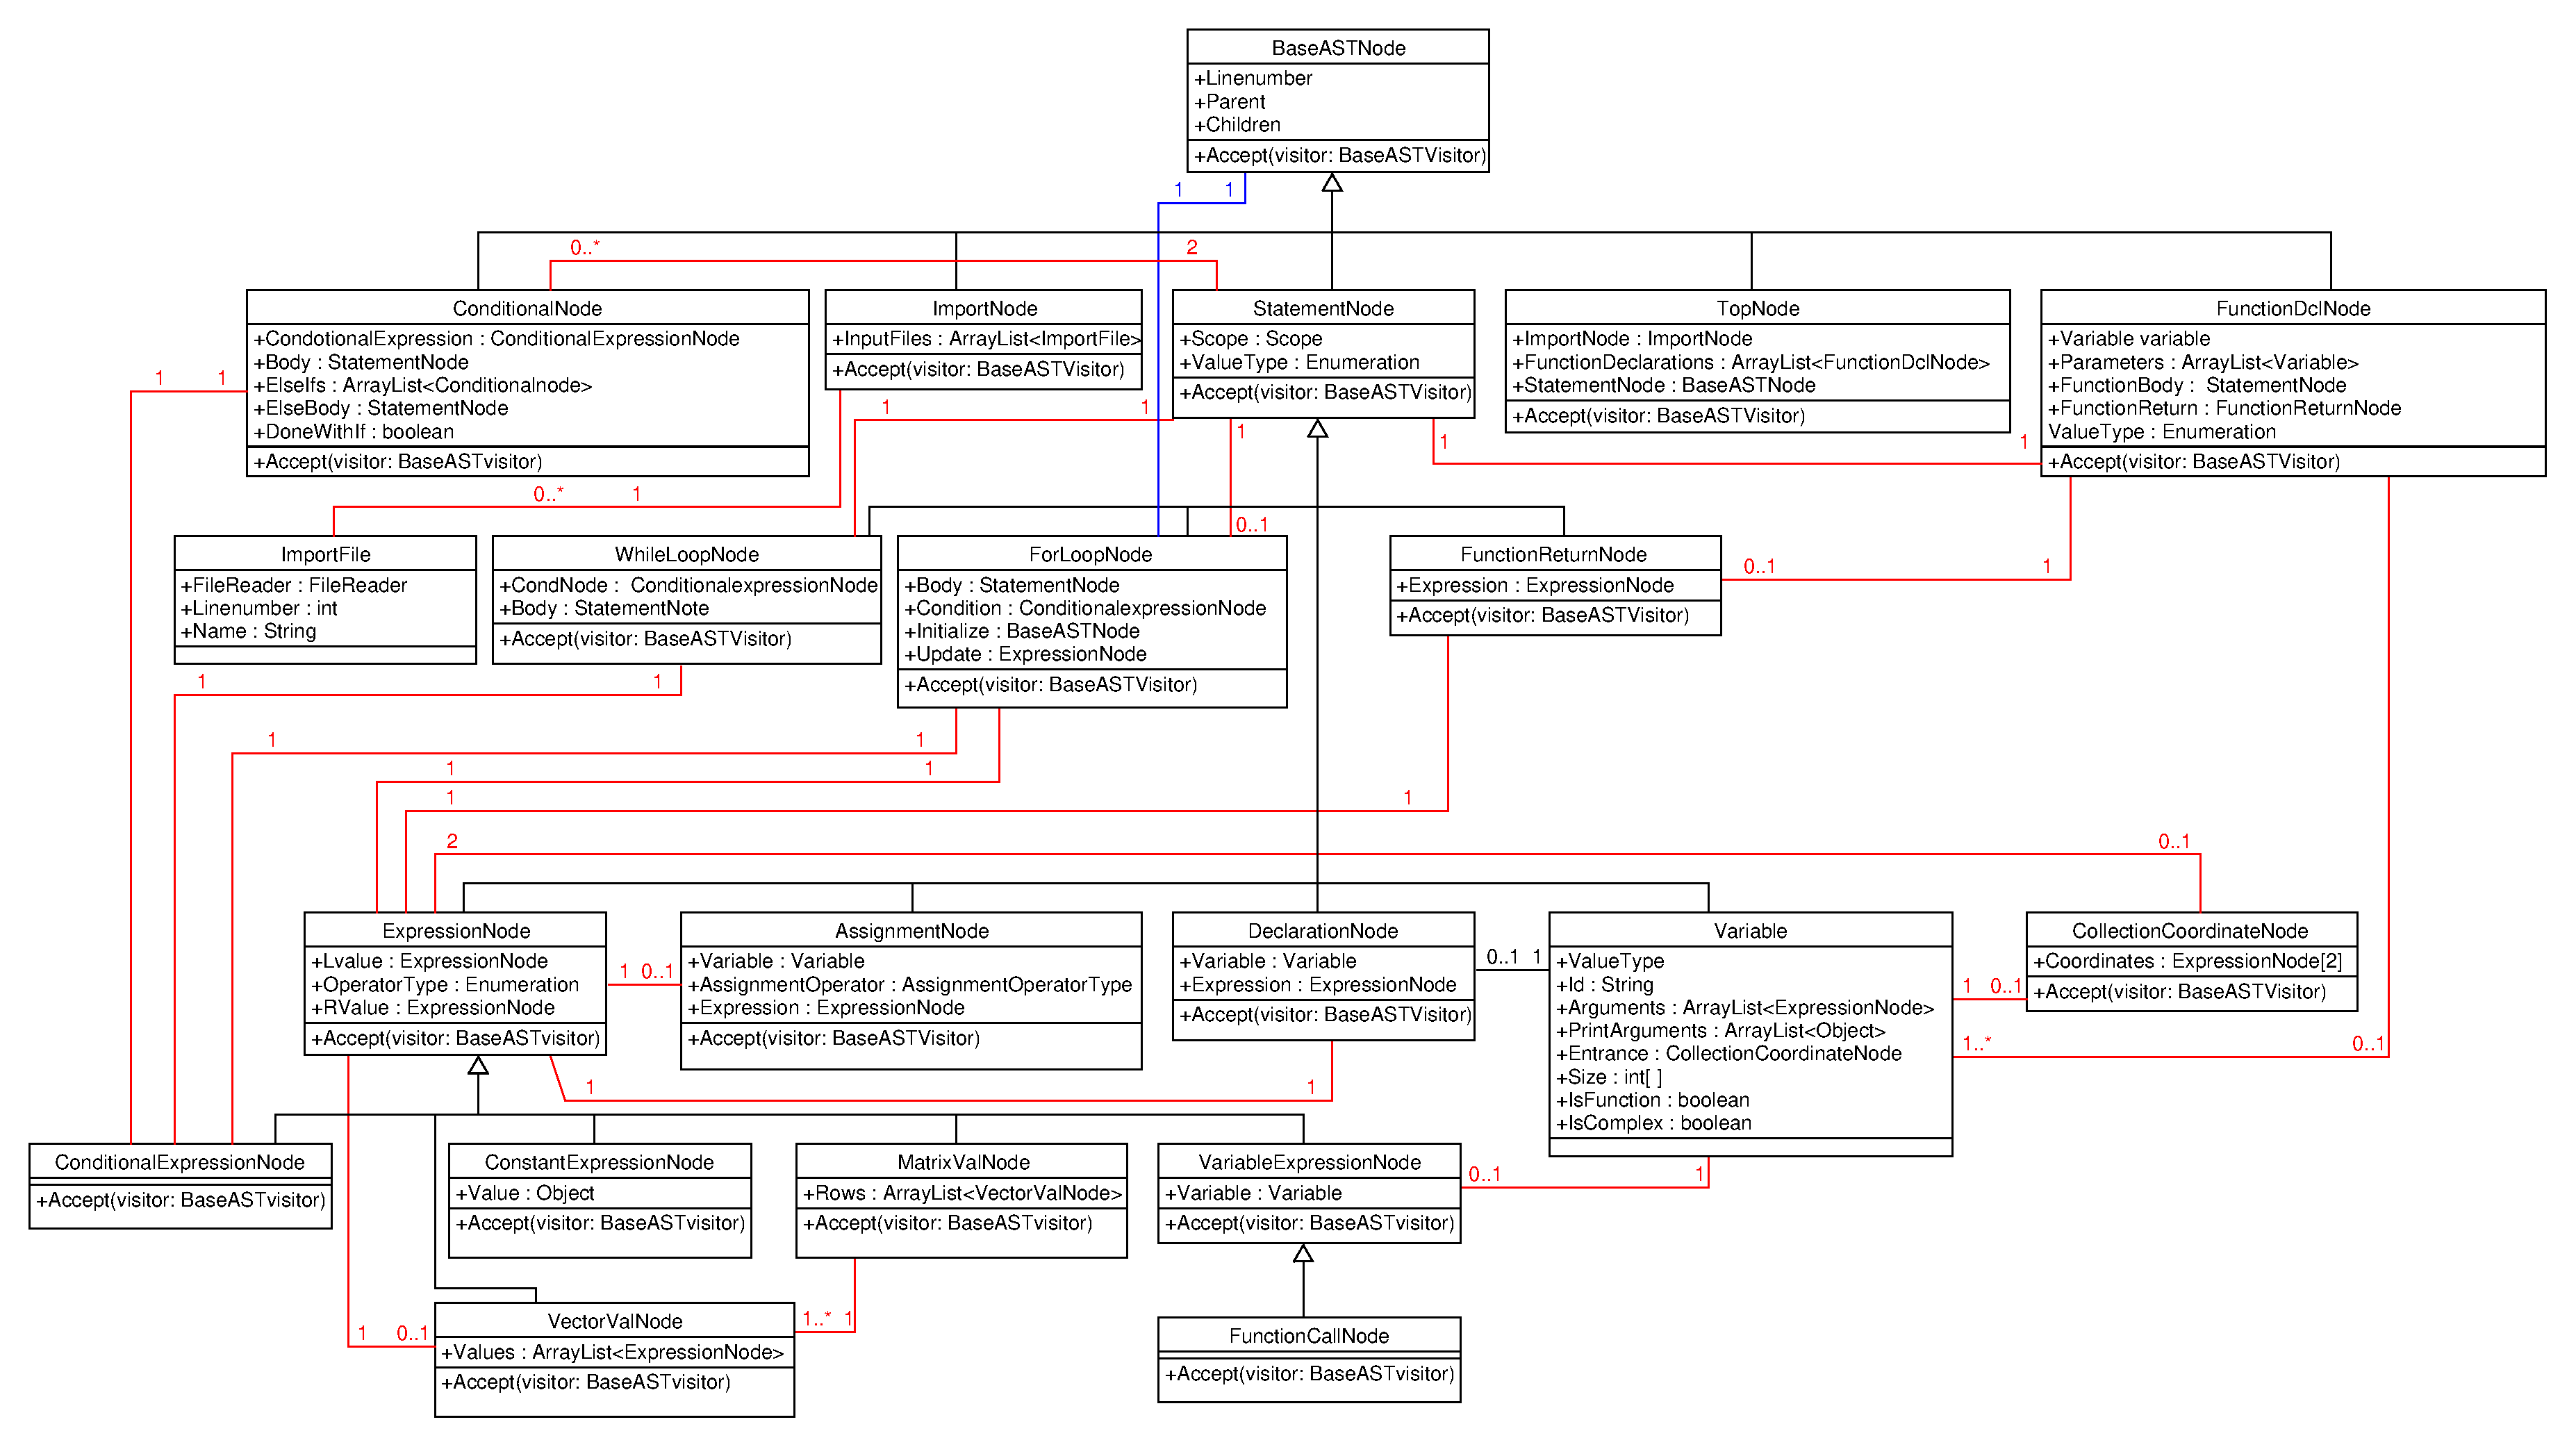
\includegraphics[scale=0.42]{figures/ClassDiagrams/ASTClassDiagram.pdf} % trim=4.85cm 15cm 0.85cm 1cm
\caption{A UML class diagram of the classes used the \acrshort{ast}.}\label{image:ASTNodes}
\vspace{-10pt}
\end{sidewaysfigure} %label app:CFG
\end{document}
